% Paper draft, Ecology and Evolution format
\documentclass[twocolumn,10pt]{article}

% encoding
\usepackage[T1]{fontenc}
\usepackage[utf8]{inputenc}

% two-column layout
\usepackage[a4paper,top=2cm,bottom=2.2cm,left=1.7cm,right=1.7cm,columnsep=0.6cm]{geometry}
\usepackage{microtype}

% fonts
\usepackage{newtxtext}
\usepackage{newtxmath}

% graphics/tables
\usepackage{graphicx}
\graphicspath{{images/}}
\usepackage{booktabs}
\usepackage{multirow}
\usepackage{array}
\usepackage{float}
\usepackage{dblfloatfix}

% colors
\usepackage{xcolor}

% bibliography style
\usepackage[round,authoryear]{natbib}
\setcitestyle{aysep={}}
\bibliographystyle{plainnat}

% section headings
\usepackage{titlesec}
\titleformat{\section}{\normalfont\bfseries}{\thesection\ \textbar\ }{0.4em}{}
\titleformat{\subsection}{\normalfont\bfseries}{\thesubsection\ \textbar\ }{0.4em}{}
\titleformat{\subsubsection}{\normalfont\bfseries\itshape}{\thesubsubsection\ \textbar\ }{0.4em}{}
\titlespacing*{\section}{0pt}{1.4ex plus .2ex}{0.6ex}
\titlespacing*{\subsection}{0pt}{1.1ex plus .2ex}{0.4ex}

% TODO macros
\newcommand{\TODO}[1]{%
  \par\medskip\noindent
  \fcolorbox{red}{yellow!15}{%
    \parbox{0.95\linewidth}{\footnotesize\textbf{\textcolor{red}{[[TODO]]}}\ #1}}%
  \par\medskip}
\newcommand{\TD}[1]{{\textbf{\textcolor{red}{[[TODO: #1]]}}}}

% captions
\usepackage{caption}
\DeclareCaptionLabelSeparator{eebar}{ \textbar\ }
\DeclareCaptionLabelFormat{eeupper}{\MakeUppercase{#1}~#2}
\captionsetup{labelformat=eeupper, labelsep=eebar, font=small, labelfont=bf}

% abstract style
\renewenvironment{abstract}{%
  \par\noindent{\normalsize\bfseries ABSTRACT}\par\vspace{0.35em}\small\noindent\ignorespaces
}{\par\vspace{0.8em}\normalsize}

% avoid overflow in narrow columns
\usepackage[htt]{hyphenat}
\usepackage{seqsplit}
\setlength{\emergencystretch}{3em}
\tolerance=2000
\hbadness=2000

% avoid stretched gaps between columns
\raggedbottom

% header/footer
\usepackage{lastpage}
\usepackage{fancyhdr}
\pagestyle{fancy}
\fancyhf{}
\renewcommand{\headrulewidth}{0.4pt}
\fancyhead[L]{\footnotesize\itshape Ecology and Evolution}
\fancyhead[R]{\footnotesize\itshape Jaguar geographic assignment via transfer learning}
\fancyfoot[C]{\footnotesize\thepage\ of \pageref{LastPage}}

% hyperref must be loaded last
\usepackage[hidelinks]{hyperref}

\begin{document}

% front matter
\twocolumn[{%
\vspace*{0.1em}
\noindent{\footnotesize\bfseries RESEARCH ARTICLE}\hfill{\footnotesize\bfseries OPEN ACCESS}\par
\vspace{0.7em}
{\raggedright\LARGE\bfseries Development of Machine Learning Models for Precise Geographic
Assignment of Jaguars (\textit{Panthera onca}) Using Complete Genomes and Transfer Learning\par}
\vspace{0.8em}
{\noindent\large Guzman Vitar\textsuperscript{1}~\TD{co-authors}\par}
\vspace{0.5em}
{\footnotesize\noindent\textsuperscript{1}\TD{affiliations}\par}
\vspace{0.5em}
{\footnotesize\noindent\textbf{Correspondence:}~\TD{corresponding-author name and email}\par}
{\footnotesize\noindent\textbf{Received:}~\textbar{}~\textbf{Revised:}~\textbar{}~\textbf{Accepted:}\par}
{\footnotesize\noindent\textbf{Funding:}~\TD{funding agencies and grant numbers}\par}
\vspace{0.5em}
{\footnotesize\noindent\textbf{Keywords:}~machine learning \textbar{} conservation genomics
\textbar{} jaguar \textbar{} geographic assignment \textbar{} transfer learning\par}
\vspace{0.9em}
\hrule
\vspace{1.2em}
}]

\begin{abstract}
Endangered species that most require precise forensic tools for anti-poaching enforcement are
typically those for which the fewest genomes are available for model development. In the jaguar
(\textit{Panthera onca}), assigning a trafficked individual to its population of origin is
constrained both by small, fragmented samples and by a feature-to-sample ratio that makes
locus selection challenging. We addressed geographic assignment from SNP data through
cross-species transfer learning. We first finetunned DNABERT-2 \citep{zhou2024dnabert} on six felid
reference assemblies, and then used the resulting foundation model to compute a label-free Variant
Effect Score (VES) for each SNP, a measure of how surprising the alternate allele is in the felid
genomic context. These scores initialized per-locus learnable gates in a genotype-matrix multilayer
perceptron, which we trained with a differentiable haversine loss to predict coordinates directly.
We evaluated every model with $55$-fold leave-one-out cross-validation over the jaguar genomes,
tuned hyperparameters by $100$-trial Optuna Bayesian search, and benchmarked against an identically
tuned no-VES control, a fixed-default Locator baseline \citep{battey2020predicting}, and the
SCAT-based assignment of \citet{lazzari2025development}. The Locator baseline reached a median
haversine error of $199$\,km, placing $67.3\%$ of individuals within $500$\,km, and the best no-VES
tuned trial reached $174$\,km, against a roughly $350$--$400$\,km SCAT reference. Introducing
VES-initialized gates improved this further: the top-$5$ trial ensemble reached $165$\,km median
haversine, while the best single Optuna trial reached $149$\,km and assigned $83.6\%$ of individuals
within $500$\,km of their true origin. Bayesian tuning and cross-species transfer thus contributed
successive gains in median error, from $199$ to $174$\,km and from $174$ to $149$\,km. These gains
were metric-dependent, however: the VES model lowered the median but not the within-$500$\,km rate,
which was highest for the tuned no-VES model ($89.1\%$) rather than for the best single VES trial
($83.6\%$). Taken together, these results show that a foundation model pre-trained across the
Felidae can supply constraint signal that a small, fragmented jaguar sample cannot provide on its
own.
\end{abstract}

% Introduction
\section{Introduction}

\TODO{Intro condensation + tense pass: the Introduction below reuses proposal literature verbatim
(jaguar conservation; conservation genomics and ML; the data-scarcity paradox; traditional methods
SCAT/SPASIBA/STRUCTURE/KLFDAPC + comparative table + Zenato Lazzari; deep-learning methods
Battey-Locator/Degen/Bayliss + comparative table; the transfer-learning promise + foundation models;
and the objectives). This is thesis-length. CONDENSE to E\&E introduction length --- keep the
jaguar/forensic motivation, the data-scarcity framing, the transfer-learning rationale, and the
objectives; trim the method-by-method literature to citations. Also run a future-tense pass on the
flagged passages (the objectives; "The innovative approach proposed here...").}

\subsection*{Jaguar Conservation}

The jaguar (Panthera onca) is the largest neotropical felid and a keystone apex predator.
Historically distributed from the southern United States to Argentine Patagonia the jaguar now
occupies only about 46\% of its original range, with an estimated 173,000 individuals
remaining—roughly half in Brazil \citep{jedrzejewski2018estimating}. Jaguars inhabit diverse
ecosystems, from dense tropical forests to wetlands, and their protection benefits numerous other
species, making them an umbrella species for biodiversity conservation.

Population status varies greatly across biomes. The Amazon and Pantanal harbor the largest, most
genetically diverse populations, with extensive connectivity and high habitat suitability. In
contrast, the Atlantic Forest and Caatinga populations are small, isolated, and genetically
impoverished due to severe fragmentation, while the Cerrado has seen a decline exceeding 50\%
\citep{haag2010effect}. Connectivity corridors, such as along the Araguaia and Paraguay Rivers, are
critical to maintain gene flow and avoid local extinctions.

Habitat loss and fragmentation remain the most severe threats. While habitat loss reduces total
area, fragmentation more acutely undermines survival by isolating populations and limiting
dispersal, especially in smaller groups. In Brazil, most jaguars now occur in protected areas, yet
many of these are too small or disconnected to ensure long-term viability. Only in the Amazon do
some reserves have sufficient size for multi-century persistence, underscoring the need for
connected protected areas and carefully planned dispersal corridors \citep{rabinowitz2010long}.

\begin{figure*}[t]
\centering
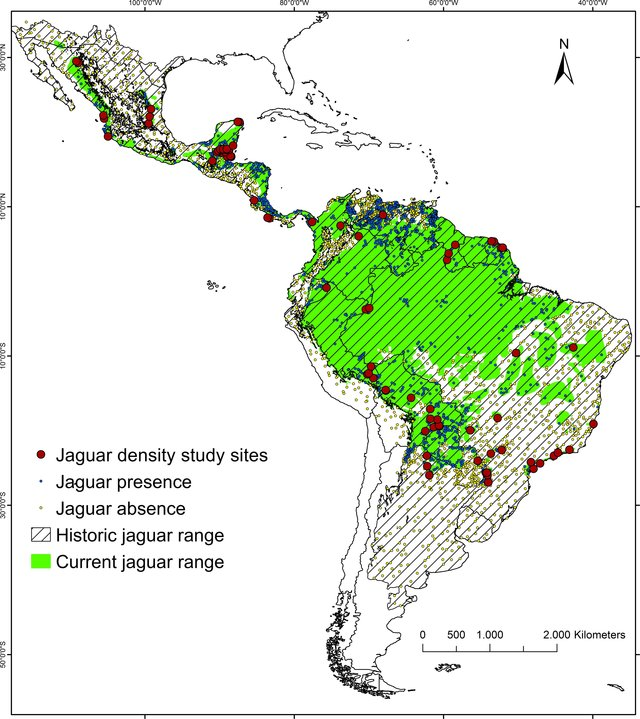
\includegraphics[width=0.7\textwidth]{images/image5.png}
\caption{Historical (light shading) and current (dark shading) distribution of the jaguar
(\textit{Panthera onca}) across the Americas. Data adapted from \citep{jedrzejewski2018estimating}.}
\label{fig:jaguar_distribution}
\end{figure*}

Human-wildlife conflict and illegal trade compound these pressures. Retaliatory killing is common
where jaguars prey on livestock, and a growing black market, driven largely by demand from Asian
countries for skins, teeth, and bones, targets populations across the Amazon and beyond
\citep{morcatty2020illegal}. Enforcement is hampered by weak governance, legal loopholes, and
clandestine trafficking networks.

A critical gap in conservation is the ability to assign poached individuals to their population of
origin, which would allow authorities to identify and prioritize anti-poaching interventions at key
hunting hotspots. Strengthening governance, enhancing forensic tools for geographic assignment,
expanding protected habitats, and disrupting trafficking routes are therefore essential for the
long-term survival of the species.

\subsection*{Conservation Genomics and Machine Learning}

A wide range of disciplines is involved in biodiversity conservation and ecosystem services.
Traditionally, genetics has helped elucidate how evolutionary processes shape genotypic and
phenotypic variation and determine the population structure of a species, in addition to identifying
potential risks related to demographic change and inbreeding on population viability. With the
advancement of genetic technology, another new field emerged, genomics, which brought a dramatic
increase in the number of genetic markers that should improve the accuracy of diversity estimates
and demographic parameters of populations relevant to conservation \citep{shafer2015genomics}.

Among the greatest contributions of genomics to conservation is the ability to predict extinction
risks and inform managers about population viability before population decline, allowing decisions
on whether translocation is a viable strategy, through the identification of loci and genomic
regions responsible for adaptation to local conditions \citep{mcmahon2014how}. Population size is
also a key factor in determining demographic viability, and this can be estimated through marker
panels designed for individual identification and kinship relationships
\citep{hohenlohe2021population}. Another area where genomic data is particularly useful and
classical genetic techniques are insufficient is the study of past population dynamics of an
endangered species – this allows us to elucidate whether the species suffered declines during its
past evolutionary history or if its current status is a consequence of what is currently happening.

Machine learning (ML) is increasingly being integrated into conservation genomics to address
complex, high-dimensional datasets. ML models can classify individuals into populations of origin,
detect cryptic population structures, and predict adaptive traits by learning patterns across
thousands or millions of genomic markers.

In addition, ML methods can be used to detect signals of selection, predict future population trends
under different environmental scenarios, and integrate genomic, environmental, and movement data for
more precise conservation planning. For example, combining genomic data with remote sensing and
ecological variables in predictive models can help identify climate-resilient habitats and forecast
range shifts. Similarly, unsupervised learning techniques such as clustering and dimensionality
reduction can reveal hidden genetic structures that may not be apparent with traditional methods,
guiding the design of protected areas and connectivity corridors.

\subsection*{The Challenge of Limited Data in Endangered Species}

A critical challenge in conservation genomics is the limited availability of genetic data for
endangered species. This scarcity stems from several factors: small population sizes, difficulties
in sample collection, ethical considerations, and the high cost of genomic sequencing. Traditional
approaches to geographic assignment and population structure analysis often require substantial
datasets to achieve reliable results, creating a paradox where the species most in need of
conservation attention have the least data available for analysis.

This limitation is particularly acute for jaguars, where population fragmentation and small sample
sizes in critical regions (such as the Atlantic Forest) make it difficult to develop robust models
for geographic assignment. While SNP-based approaches have provided valuable insights, they often
require large numbers of individuals per population to achieve sufficient precision, especially when
dealing with subtle genetic differentiation between recently fragmented populations
\citep{lazzari2025development, haag2010effect}.

The core challenge addressed by this project is the fundamental paradox in conservation genomics:
endangered species, which require the most precise genetic tools for their protection, often have
the least genetic data available for analysis. Traditional approaches to geographic assignment
require substantial sample sizes per population to achieve reliable results, creating a significant
barrier for species like jaguars where populations are small, fragmented, and difficult to sample
\citep{shafer2015genomics}.

\subsection*{Traditional Statistical Methods for Geographic Assignment}

The scientific challenge of assigning individuals to their geographic origin based on genetic data
predates the current wave of machine learning. Classical approaches were built on population
genetics theory, statistical modeling, and multivariate analysis. These methods remain foundational
in conservation genetics and wildlife forensics, providing the first rigorous frameworks for linking
DNA variation to geography. Four representative approaches—SCAT, SPASIBA, STRUCTURE and
KLFDAPC—illustrate the logic behind traditional assignment methods.

\paragraph{SCAT – Smoothed and Continuous Assignment Tests}

The development of SCAT by Wasser and colleagues (2004) \citep{wasser2004assigning} marked a turning
point in applying genetics to wildlife forensics. The core idea of SCAT is to model allele
frequencies as continuous surfaces across geographic space rather than discrete population
boundaries. By using microsatellite markers from African elephants, SCAT estimated allele frequency
gradients through spatial smoothing and then calculated likelihood surfaces for each individual's
genotype. This probabilistic framework allowed researchers to infer the most likely geographic
origin of ivory samples, even in regions where reference samples were sparse.

The strength of SCAT lies in its ability to interpolate beyond sampled locations, producing
continuous assignment maps rather than binary classifications. This was particularly powerful in
identifying poaching hotspots in Africa, where many areas lacked dense sampling. Results showed that
50\% of samples were assigned within roughly 500 km of their true origin, and resolution improved
substantially in well-sampled regions, sometimes below 200 km. However, the method was
computationally intensive, requiring Markov Chain Monte Carlo (MCMC) to approximate posterior
distributions, and its accuracy decreased markedly in under-sampled regions. Despite these
challenges, SCAT established the feasibility of continuous geographic assignment from limited
genetic markers and became a cornerstone for forensic applications.

\paragraph{SPASIBA – Spatial Bayesian Inference}

Building on the ideas of SCAT, Guillot and colleagues (2016) \citep{guillot2016accurate} developed
SPASIBA, a method designed to improve computational efficiency and extend applicability to
genome-scale SNP data. SPASIBA treats allele frequencies as spatially autocorrelated random fields,
with covariance decaying as geographic distance increases. Instead of relying on MCMC, SPASIBA uses
Integrated Nested Laplace Approximation (INLA), a deterministic Bayesian inference method that is
far faster and more scalable. This makes it practical to analyze larger datasets with hundreds or
thousands of SNPs.

SPASIBA has been applied successfully to a range of taxa, including Florida scrub-jays and
\textit{Arabidopsis thaliana}. In the scrub-jay study, using 41 SNPs, SPASIBA localized individuals
with a median error of about 26 km, demonstrating impressive resolution at fine scales. In
\textit{Arabidopsis}, with 1000 SNPs, the method achieved 75th-percentile errors of around 93 km
across the species' European range. These results show that SPASIBA can exploit genome-wide SNP data
to generate highly accurate predictions, while also producing probabilistic maps similar to SCAT.
Nevertheless, the method assumes Hardy–Weinberg and linkage equilibrium, and like SCAT, its accuracy
still depends heavily on reference sampling density. Its computational demands are lower than SCAT's
but still non-trivial, requiring specialized software and statistical expertise.

\paragraph{STRUCTURE – Bayesian Clustering for Population Assignment}

STRUCTURE \citep{pritchard2000inference} implements a Bayesian clustering framework that infers
population structure directly from multilocus genotype data without requiring prior knowledge of
individual origins. The model assumes Hardy–Weinberg and linkage equilibrium within populations and
uses Markov Chain Monte Carlo (MCMC) sampling to assign individuals probabilistically to \textit{K}
genetic clusters. Each individual receives a vector of membership coefficients, representing the
proportion of its genome originating from each cluster, which allows the detection of both discrete
population boundaries and admixture.

In practice, STRUCTURE has been widely applied in conservation genetics to identify distinct
populations, measure gene flow, and assign individuals of unknown origin to their most likely
population. A critical advantage is its ability to reveal hidden structure: clusters can emerge from
the genetic data even when population boundaries are not obvious in the field.

Despite its impact, STRUCTURE has limitations. The method produces clusters rather than explicit
spatial coordinates, so its geographic resolution is constrained to population-level inferences. The
accuracy of assignments depends on the value of \textit{K}, which must be chosen carefully.
Computational cost can also be high for large SNP datasets, though faster variants and related
programs such as BAPS and GENELAND have attempted to address this. Moreover, performance declines
when populations are weakly differentiated or when reference sampling is sparse.

Nevertheless, STRUCTURE remains a cornerstone in conservation genomics. Its probabilistic framework
and ability to detect admixture have made it the default method for many population-level assignment
studies. As such, it provides both a conceptual and practical foundation against which newer spatial
and machine learning approaches can be compared.

\paragraph{KLFDAPC – Kernel Local Fisher Discriminant Analysis of Principal Components}

A different branch of approaches focuses on discriminating individuals among predefined populations.
One widely used framework is discriminant analysis of principal components (DAPC), which uses PCA
for dimensionality reduction followed by linear discriminant analysis to maximize group separation.
While DAPC has proven useful, it is inherently linear and may fail to capture nonlinear genetic
relationships shaped by geography.

Qin and colleagues (2022) \citep{qin2022klfdapc} addressed this limitation with KLFDAPC, which
incorporates kernel methods into the Fisher discriminant framework applied to PCA-transformed data.
By embedding data in a nonlinear feature space, KLFDAPC can separate populations that overlap in
linear PCA space but differ along nonlinear axes of genetic variation. Applied to both simulations
and human SNP datasets, KLFDAPC recovered geographic structures more faithfully than PCA or DAPC,
improving classification accuracy and producing axes more consistent with known geography. The
method requires labeled reference populations and therefore does not produce continuous spatial
assignments like SCAT or SPASIBA. Instead, it excels in cases where discrete populations can be
defined and sampled.

\begin{table*}[t]
\centering
\caption{Comparison of traditional methods for geographic assignment}
\label{tab:traditional_methods}
\small
\begin{tabular}{p{1.8cm}p{2.3cm}p{2cm}p{1.5cm}p{2.5cm}p{2.5cm}}
\hline
\textbf{Method}
  & \textbf{Input Data}
  & \textbf{Output Type}
  & \textbf{Comp. Cost}
  & \textbf{Strengths}
  & \textbf{Weaknesses} \\
\hline
SCAT
  & Geo-tagged genetic data, continuous allele frequencies
  & Continuous origin estimates
  & Moderate-high
  & Good for fine spatial gradients, continuous mapping
  & Sensitive to sampling density, assumptions about dispersal \\
\hline
SPASIBA
  & SNP / genotype data + spatial coordinates
  & Continuous geographic assignment
  & High
  & Provides high resolution continuous estimates
  & Computationally intensive, requires many samples \\
\hline
STRUCTURE
  & Multilocus genotype data, no spatial info built in
  & Assigns individuals to discrete clusters
  & Moderate
  & Captures population structure, widely used
  & Coarse, less precise for continuous geography \\
\hline
KLFDAPC
  & Genotypes + optional geography, dimension reduction \& clustering
  & Discrete or semi-continuous assignment
  & Moderate
  & Can combine spatial smoothing \& allele frequency variation
  & Less interpretable, may miss fine-scale continuous gradient \\
\hline
\end{tabular}
\end{table*}

\paragraph{Jaguar geographical assignment}

In 2025, Zenato Lazzari and colleagues \citep{lazzari2025development} applied various genomic
methods specifically for jaguar conservation, developing a species-specific SNP panel to facilitate
geographic assignment. Their study combined whole-genome sequencing with a suite of population
genetic tools to create both a full and reduced panel of highly informative SNPs.

The dataset comprised 58 whole genomes representing jaguars from all five Brazilian biomes: Amazon,
Pantanal, Atlantic Forest, Cerrado, and Caatinga. From this, they identified candidate SNPs and
selected loci based on pairwise F\_ST values, maximizing their ability to distinguish between
regional populations. The final design produced the Jag-SNP panel of 459 loci, along with a reduced
84-SNP panel optimized for cost-effectiveness.

To assess performance, the authors used principal component analysis (PCA) to visualize genetic
differentiation among individuals from the five biomes and to confirm that the selected SNPs
captured population structure. Assignment accuracy was then tested using likelihood-based
statistical frameworks. Approximately 98\% of individuals were correctly assigned to their biome of
origin, and 65–69\% could be localized within 500 km of their actual sampling site. Interestingly,
the highest accuracy occurred in isolated populations with reduced genetic diversity, while
continuous habitats such as the Amazon showed lower resolution due to high gene flow and correlated
allele frequencies.

Overall, the Jaguar SNP panel demonstrates how combining genome-wide data, F\_ST-based marker
selection, PCA validation, and likelihood-based assignment tests can yield a robust and
cost-efficient forensic tool for conservation.

Geographic assignment of individuals based on genetic data is an important task in conservation
genomics, particularly for forensic applications aimed at combating poaching and illegal trade.

Traditional approaches, such as PCA or Bayesian clustering, have provided valuable insights but
often require large sample sizes and struggle with subtle differentiation across fragmented
populations.

In recent years, machine learning methods, ranging from kernel-based dimensionality reduction to
deep learning, have emerged as powerful alternatives to traditional methods. These approaches
improve accuracy, scalability, and the ability to capture non-linear patterns in genomic data.

\subsection*{Deep Learning for Geographical Assignment \& Genetic Data Representation}

\paragraph{Battey et al – Locator: Deep Neural Network for Geographic Assignment}

Battey and colleagues (2020) \citep{battey2020predicting} set out to address the limitations of
traditional Bayesian geographic assignment models, which, while powerful, are computationally
expensive and often struggle with fine-scale resolution.

Their goal was to explore whether deep neural networks could offer both greater accuracy and
efficiency by directly predicting the geographic coordinates of individuals from their genomic data.
By reframing the problem as a regression task, they aimed to capture subtle spatial allele frequency
patterns that classical models often miss.

To implement this, the authors designed a fully connected feedforward neural network architecture,
essentially a multilayer perceptron (MLP). The input layer took thousands of SNP-derived genotypes
encoded as numerical features, which were then passed through several hidden layers with nonlinear
activation functions (ReLU) to model complex interactions among alleles. Dropout layers were
included to reduce overfitting, and the output layer consisted of two continuous nodes representing
latitude and longitude, optimized with Euclidean distance loss between predicted and true
coordinates. This relatively simple but powerful architecture allowed Locator to generalize across
genomic windows and datasets, balancing predictive capacity with computational efficiency.

To test their approach, the authors applied their model, Locator, to both simulated and empirical
data. The simulated datasets provided controlled scenarios where the true spatial origin of each
individual was known, allowing for a rigorous assessment of accuracy.

For empirical validation, they used whole-genome sequencing data from a diverse set of systems:
Anopheles mosquitoes sampled across Africa, Plasmodium falciparum parasites from Africa and Asia,
and global human genomic datasets. This range of datasets was critical, as it tested the method's
robustness under varying marker densities, levels of population structure, and geographic scales.

The results demonstrated that the neural network not only outperformed the Bayesian comparator
SPASIBA in terms of speed but also achieved strikingly higher accuracy. Locator localized
individuals to within approximately four dispersal generations in simulated data, while in empirical
datasets median assignment errors ranged from only 5.7 km in mosquitoes to about 85 km in Plasmodium
and human populations. Importantly, the runtime improvements were substantial, with Locator
operating an order of magnitude faster than SPASIBA, making it suitable for genome-wide
applications.

Despite these advances, the study highlighted two key limitations: the model's dependence on large,
representative training datasets and its black-box nature, which obscures the biological
interpretation of the features driving predictions.

\paragraph{Degen et al – Comparing Machine Learning Approaches for Continuous Spatial Assignment}

Degen and colleagues (2025) \citep{degen2025machine} investigated whether modern machine learning
approaches could improve the continuous geographic assignment of individuals from SNP data in
European tree species. Their goal was to benchmark several methods against each other, including
deep learning, Gaussian process regression (GPR), k-nearest neighbors, and genomic best linear
unbiased prediction (GBLUP).

The deep learning component was built around a multilayer perceptron (MLP) similar in spirit to
Battey et al.'s Locator, but optimized for continuous regression of geographic coordinates. Genotype
features (SNPs) were passed into a network of dense hidden layers with nonlinear activations,
designed to capture allele frequency gradients and complex dependencies between loci.
Hyperparameters such as layer depth, number of units per layer, and dropout rates were tuned to
balance generalization with predictive performance. The output layer produced two continuous values
for latitude and longitude, again trained with a regression loss function that minimized the
Euclidean distance between predicted and true coordinates. This allowed the DNN to flexibly model
nonlinear genotype–geography relationships, while complementing GPR, which excelled at uncertainty
estimation.

The datasets used were SNP panels from two widespread species: European beech (\textit{Fagus
sylvatica}) and European oak (\textit{Quercus robur}). Both species were sampled broadly across
their ranges, providing thousands of individuals with known geographic origins. These large datasets
offered an opportunity to test whether machine learning could recover fine-scale population
structure and spatial gradients of allele frequencies that reflect evolutionary and demographic
processes.

Results revealed that both deep neural networks (multi-layer perceptrons) and GPR with a Matérn
kernel achieved the highest accuracy, predicting origins with median errors of $\sim$55–76 km for
beech and $\sim$263–278 km for oak. These errors were substantially smaller than those achieved by
simpler models like k-NN or GBLUP.

The authors noted that GPR provided probabilistic uncertainty estimates, which are useful in
practice, while DNNs were more flexible in modeling nonlinear interactions between SNPs. Both
methods required large amounts of training data and computational resources.

\paragraph{Bayliss et al. - Hierarchical ML for Geographic Assignment of Genomic Samples}

A recent preprint by Bayliss et al. (2023) \citep{bayliss2022hierarchical} introduces a hierarchical
machine learning framework for predicting the geographic origin of genomic samples, with Salmonella
enterica serovar Enteritidis as the proof of concept. The aim is to trace sources of infection by
assigning each genome to its most likely continent, sub-region, and country of origin directly from
DNA data. Rather than relying on deep neural networks, the authors explored more classical ML
approaches such as random forests, gradient boosting, and support vector machines, demonstrating the
strength of these methods in large-scale genomic inference.

The dataset consisted of 2,313 S. Enteritidis genomes collected by the UK Health Security Agency
between 2014 and 2019, each linked to one of 53 geographic classes organized hierarchically: four
continents, eleven sub-regions, and thirty-eight countries. Instead of training a single flat
classifier, the researchers implemented a ``local classifier per node" strategy, cascading models so
that predictions flowed from continent to sub-region to country. This design reduced
misclassifications by ensuring that finer-level predictions were restricted to plausible sub-areas
once higher-level categories were determined.

Genetic features were extracted from sequencing data using k-mer units, and multiple algorithms were
systematically evaluated under consistent conditions. The team tested random forests, SVMs,
k-nearest neighbors, XGBoost, and Naïve Bayes, while carefully addressing class imbalance with
resampling techniques and reducing feature dimensionality through iterative selection based on
random forest importance scores. Ultimately, optimized random forests were selected at each
hierarchical level, striking a balance between predictive accuracy, interpretability, and
computational speed. The resulting pipeline could analyze raw reads and deliver a geographic
prediction in under four minutes—a stark contrast with more labor-intensive phylogeographic
analyses.

The results were compelling. At the continental level, accuracy was extremely high (macro F1
$\approx$ 0.954). Performance remained strong at the sub-regional level (F1 $\approx$ 0.718) and
reached a respectable macro F1 of 0.661 at the country level, even across 38 classes. In practice,
some countries—particularly those with high travel links to the UK—achieved hierarchical F1 scores
above 0.90, reflecting near-perfect precision. Crucially, the method generalized well: when applied
to external Salmonella datasets outside the original training set, accuracy remained robust,
indicating that the models captured true geographic signals in the genomes rather than simply
memorizing the data.

The novelty of this work lies in showing that established ensemble methods, implemented
hierarchically, can deliver accurate, fine-scale geographic predictions from genomic data without
the heavy computational demands of deep learning. Bayliss et al.'s approach enriches the
methodological toolkit for geographic assignment, complementing deep-learning tools like Locator and
Gaussian-process models with a practical, transparent, and efficient alternative.

\begin{table*}[t]
\centering
\caption{Comparison of machine learning approaches for geographic assignment}
\label{tab:ml_methods_comparison}
\small
\begin{tabular}{p{2.5cm}p{2.5cm}p{2.5cm}p{2.5cm}p{2.5cm}}
\hline
\textbf{Study} & \textbf{Goals} & \textbf{Methods} & \textbf{Results} & \textbf{Limitations} \\
\hline
Battey et al. (2020)
  & Improve speed and accuracy of geographic assignment
  & Deep neural network (Locator) predicting coordinates
  & Median errors 5.7–85 km; 10× faster than Bayesian models
  & Requires large datasets; limited interpretability \\
\hline
Degen et al. (2025)
  & Benchmark ML models for continuous assignment
  & DNNs, GPR, k-NN, GBLUP
  & DNN and GPR: 55–76 km (beech), 263–278 km (oak)
  & High computational demands; requires large datasets \\
\hline
Bayliss et al. (2022)
  & Hierarchical geographic assignment
  & Random Forests, SVMs, XGBoost (hierarchical)
  & F1: 0.954 (continent), 0.718 (sub-region), 0.661 (country)
  & Performance drops at finer scales; requires substantial data \\
\hline

\end{tabular}
\end{table*}

\subsection*{The Promise of Transfer Learning in Conservation Genomics}

Recent advances in machine learning, particularly in the field of natural language processing, have
introduced powerful techniques for learning from limited data through transfer learning. These
approaches allow models pre-trained on large, general datasets to be fine-tuned for specific tasks
with much smaller datasets, often achieving superior performance compared to models trained from
scratch.

In the context of genomics, foundation models like DNABERT-2 \citep{zhou2024dnabert} have
demonstrated remarkable capabilities in understanding DNA sequence patterns across multiple species.
These models can capture complex genomic features and relationships that may not be apparent through
traditional analytical methods. By leveraging the knowledge learned from large, diverse genomic
datasets, these models can potentially overcome the data scarcity challenges faced in endangered
species conservation.

Recent developments in genomic machine learning have introduced foundation models, which are
large-scale pre-trained architectures designed to capture universal features of DNA sequences across
species. These models—such as \textbf{DNABERT-2} \citep{zhou2024dnabert} and the \textbf{Nucleotide
Transformer} (Dalla-Torre et al., 2025) \citep{dallatorre2025nucleotide}—represent a paradigm shift
in the field. Their goal is to learn rich, generalizable representations of nucleotide sequences
that can be transferred to diverse downstream tasks, from variant effect prediction to motif
discovery, often with minimal fine-tuning data.

The results have been striking. Both DNABERT-2 and the Nucleotide Transformer achieve
state-of-the-art performance across a wide range of genomic benchmarks. DNABERT-2, for instance,
outperforms classical CNNs and RNNs on promoter prediction, transcription factor binding site
recognition, and splice site identification, often by large margins \citep{zhou2024dnabert}.
Similarly, the Nucleotide Transformer has shown that pretraining across many species enables
cross-species transfer, where a model trained on non-human genomes can still perform strongly on
human tasks \citep{dallatorre2025nucleotide}.

\begin{figure*}[t]
\centering
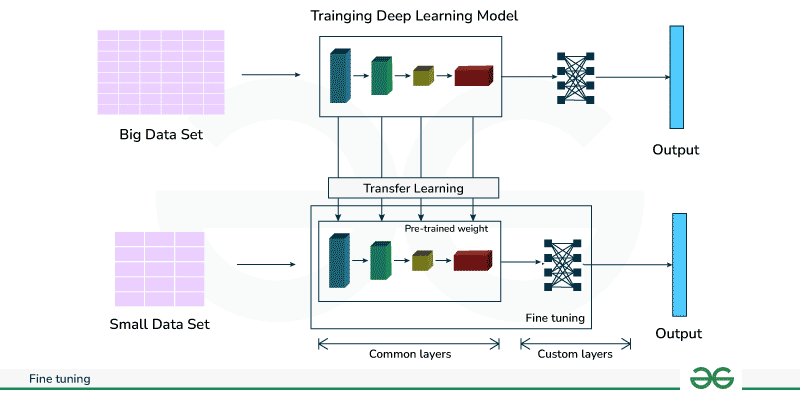
\includegraphics[width=0.9\textwidth]{images/image1.png}
\caption{Illustration of transfer learning and fine-tuning : a pre-trained base model's shared
layers are reused, while task-specific layers are added and trained on the target dataset.
Understanding Fine-Tuning of Large Language Models (LLMs) : Instruction Tuning and Beyond (Medium,
2023).}
\label{fig:illustration_transfer_learning_and_finetuning}
\end{figure*}

The innovative approach proposed here leverages the power of transfer learning in machine learning
to overcome this data scarcity challenge. By pre-training a foundation model on comprehensive feline
genomic data and then fine-tuning it on jaguar-specific sequences, we can potentially achieve levels
of precision and reliability that were previously unattainable with traditional methods. This
approach represents a paradigm shift in conservation genomics, moving from methods that require
large datasets to methods that can work effectively with limited data through the power of
pre-trained models.

\subsection*{OBJECTIVES}

\paragraph{General Objective}

Develop and evaluate a machine learning pipeline using transfer learning and foundation models for
precise geographic assignment of jaguars (\textit{Panthera onca}) from different Brazilian biomes,
overcoming the limitations of limited genetic data through pre-training on comprehensive feline
genomic datasets.

\paragraph{Specific Objectives}

\begin{enumerate}
        \item Pre-train a DNABERT-2 foundation model on comprehensive feline genomic data from the
Darwin's Ark database to learn general patterns of genomic variation across felid species;
        \item Fine-tune the pre-trained model on complete jaguar genomes from different Brazilian
biomes to develop a specialized model for jaguar geographic assignment;
        \item Evaluate the performance of the transfer learning approach compared to traditional
methods for geographic assignment, particularly in scenarios with limited sample sizes;
        \item Develop a computational pipeline for automated geographic assignment of jaguar samples
of unknown origin, with applications in forensic analysis and conservation management;
        \item Assess the model's ability to identify subtle genetic differentiation between recently
fragmented populations, particularly in the Atlantic Forest biome where sample sizes are critically
small.
\end{enumerate}

% Materials and Methods
\section{Materials and Methods}

\subsection{Foundation Model: DNABERT-2}

We will employ the DNABERT-2 architecture as our foundation model, which represents the current
state-of-the-art in genomic language modeling \citep{zhou2024dnabert}.

The model incorporates several advanced architectural features designed to handle the specific
complexities of genomic data. Central to its design is Attention with Linear Biases (ALiBi), a
mechanism that allows the model to extrapolate to longer input sequences than those seen during
training, effectively bypassing the limitations of traditional learned positional embeddings.
Furthermore, the integration of Flash Attention drastically improves memory usage and computational
speed during both training and inference phases. These optimizations, combined with its inherent
multi-species pre-training capability, allow DNABERT-2 to learn robust, generalizable patterns
across diverse genomic datasets before specific adaptation.

\subsection{Felid Foundation Pre-training Corpus}
We assembled the felid foundation pre-training corpus from six reference genome assemblies spanning
three genera of the family Felidae, chosen so that the jaguar (\textit{Panthera onca}) sits within a
phylogenetically broad but taxonomically focused sample of its own family rather than within a
generic vertebrate mixture. The roster is closed and pinned in code: each entry fixes the species
binomial, an assembly identifier, the assembly name, and the NCBI taxonomy identifier, and adding a
species requires an explicit code and test change, so that the corpus cannot silently drift between
runs. Five of the six assemblies were drawn from NCBI RefSeq and downloaded from the canonical
RefSeq FTP tree; the jaguar assembly was taken from the DNA Zoo Hi-C submission
(\texttt{Panthera\_onca\_HiC}) through a pinned direct URL, with a HuggingFace mirror as a secondary
source. Every compressed FASTA was integrity-checked at download time against a manually pinned
checksum --- MD5 for the RefSeq files and SHA-256 for the jaguar DNA Zoo file --- so that a
truncated or stale payload is rejected rather than silently ingested. Table~\ref{tab:felid-corpus}
lists the six assemblies together with the number of $512$~bp windows each contributed to the
corpus.

\begin{table*}[t]
\centering
\caption{The six felid reference assemblies in the foundation pre-training corpus. Windows are the
number of tokenised $512$~bp windows contributed to the train and validation folds; species are
listed in the identifier-sorted registry order used by the pipeline.}
\label{tab:felid-corpus}
\begin{tabular}{llllrr}
\toprule
Species & Common name & Identifier & Assembly & Train & Validation \\
& & & & windows & windows \\
\midrule
\textit{Panthera onca}
  & Jaguar
  & \texttt{DNAZOO\_Panthera\_onca\_HiC}
  & \texttt{Panthera\_onca\_HiC}
  & 4{,}822{,}435
  & 1{,}217{,}303 \\
\textit{Felis catus}
  & Domestic cat
  & \texttt{GCF\_000181335.3}
  & \texttt{Felis\_catus\_9.0}
  & 5{,}014{,}368
  & 1{,}264{,}395 \\
\textit{Panthera tigris}
  & Amur tiger
  & \texttt{GCF\_000464555.1}
  & \texttt{PanTig1.0}
  & 4{,}384{,}605
  & 1{,}105{,}029 \\
\textit{Panthera pardus}
  & Leopard
  & \texttt{GCF\_001857705.1}
  & \texttt{PanPar1.0}
  & 4{,}240{,}897
  & 1{,}080{,}228 \\
\textit{Puma concolor}
  & Puma
  & \texttt{GCF\_003327715.1}
  & \texttt{PumCon1.0}
  & 3{,}763{,}602
  & 935{,}831 \\
\textit{Panthera leo}
  & Lion
  & \texttt{GCF\_018350215.1}
  & \texttt{P.leo\_Ple1\_pat1.1}
  & 4{,}739{,}028
  & 1{,}188{,}593 \\
\midrule
\multicolumn{4}{r}{Total} & 26{,}964{,}935 & 6{,}791{,}379 \\
\bottomrule
\end{tabular}
\end{table*}

The corpus was built directly from the reference FASTA files, with no variant-calling or consensus
step: we emitted one sequence record per contig, tagged with a provenance label of
\texttt{reference} and a species slug (for example \texttt{panthera\_onca}) that identifies its
source assembly. Each contig sequence was first normalised by upper-casing and validating it against
the fixed nucleotide alphabet $\{\mathrm{A},\mathrm{C},\mathrm{G},\mathrm{T},\mathrm{N}\}$; because
the foundation configuration pins the unsupported-symbol policy to \texttt{reject}, any character
outside this alphabet aborts the run rather than being coerced, so that no out-of-alphabet base can
leak into a training window. Contigs shorter than the $512$~bp context window were dropped as short
sequences before windowing; together with the ambiguity filter, this reduced the jaguar Hi-C
assembly from $410{,}593$ contigs to $67{,}420$ windowing-eligible sequences.

We then slid a fixed $512$~bp window along each retained contig with a stride of $384$~bp --- that
is, a $128$~bp overlap between consecutive windows --- which provides coverage of window-boundary
regions while bounding the total corpus size. Windows were never $\mathrm{N}$-padded at contig ends:
any trailing fragment shorter than $512$~bp was discarded rather than padded, so that every emitted
window is exactly $512$~bp of real sequence. As a further quality filter we required each window to
contain at most a $5\%$ fraction of ambiguous ($\mathrm{N}$) bases, discarding those that exceeded
this threshold. This procedure produced $33{,}756{,}314$ tokenised windows in total across the six
assemblies.

Each retained window was tokenised with the DNABERT-2 byte-pair-encoding (BPE) tokenizer
\citep{zhou2024dnabert}, loaded from the HuggingFace model \texttt{zhihan1996/DNABERT-2-117M} and
pinned to the immutable Git revision \texttt{\seqsplit{7bce263b15377fc15361f52cfab88f8b586abda0}} so
that the tokenisation is exactly reproducible; as DNABERT-2's custom implementation requires, the
tokenizer was loaded with \texttt{trust\_remote\_code} enabled. Tokenisation added the model's
special tokens and, rather than truncating, asserted that no window exceeded the model's maximum
position-embedding length of $512$ tokens, so that any window whose BPE encoding overflowed the
context would fail loudly instead of being silently clipped. The tokenised windows were written to a
partitioned Parquet corpus keyed by (split, contig, block), each window carrying its genomic
coordinates and a SHA-256 hash of its nucleotide string, so that any window can later be audited
against its source assembly without re-reading the original FASTA. To keep peak memory bounded on
the six multi-gigabase assemblies, each species was processed independently and streamed to the
writer in fixed-size chunks, and a cross-species contig-name collision check guaranteed that the
shared \texttt{contig:block\_start-block\_end} locus namespace never aliases windows from different
assemblies.

Train and validation folds were assigned in a locus-safe manner that eliminates leakage between
overlapping windows. Before windowing, each assembly's coordinate space was partitioned into
contiguous $50$~kb locus blocks, and every block was assigned deterministically to a fold by hashing
its locus identifier: we computed a SHA-256 digest of the string
\texttt{feline-locus-split-v1:\{locus\_id\}}, mapped its leading $64$ bits into $[0,1)$, and applied
an $80\%/20\%$ cumulative-weight cutoff to route the block to either train or validation. Because
every window inherits the split of the single $50$~kb block that contains it, and the $50$~kb block
size comfortably exceeds the $512$~bp window length, no two overlapping windows can ever straddle
the train/validation boundary; the pipeline additionally asserts this invariant explicitly, raising
a hard error if any locus maps to two folds or if overlapping windows on the same contig receive
different folds. The $50$~kb block also exceeds the autocorrelation length of most local genomic
features, so that the validation fold measures generalisation to genuinely unseen loci rather than
to shifted copies of training windows. The resulting global split placed $26{,}964{,}935$ windows
($79.9\%$) in the training fold and $6{,}791{,}379$ ($20.1\%$) in the validation fold.

We then adapted DNABERT-2 to the felid corpus by continued masked-language-modelling (MLM)
pre-training, warm-starting from the same pinned \texttt{zhihan1996/DNABERT-2-117M} checkpoint and
revision and loading it through \texttt{AutoModelForMaskedLM} so that the MLM prediction head was
available. Following the standard MLM objective, $15\%$ of tokens were masked dynamically in every
batch by a data collator --- a fresh random mask at each step --- and the model was trained to
recover the original tokens from their surrounding context. Training used bfloat16 (bf16) mixed
precision under \texttt{accelerate} together with the AdamW optimizer \citep{kingma2014adam}, with
decoupled weight decay of $0.01$ applied to all parameters except biases and LayerNorm weights, an
initial learning rate of $5\times10^{-5}$ --- a conservative rate appropriate for continued rather
than from-scratch pre-training --- and a cosine-annealing schedule preceded by a $500$-step linear
warmup. Because DNABERT-2 ships without a padding token, we set the pad token to the existing
end-of-sequence token. DNABERT-2's Triton flash-attention kernel was disabled at load time, as it is
incompatible with the installed Triton version, and the model fell back to the standard PyTorch
attention path. The remaining optimisation settings are collected in
Table~\ref{tab:felid-pretrain-hparams}; the effective batch size is $32\times2\times W$ sequences,
where $W$ is the number of data-parallel processes. Under this schedule the run reached its best
validation MLM cross-entropy loss of $4.278$ at step $36{,}000$ --- a validation perplexity of
approximately $72$ --- with the most recent recorded checkpoint at step $40{,}000$ and an
early-stopping patience counter of four out of five, that is, four consecutive $1{,}000$-step
evaluation cycles without improvement over the step-$36{,}000$ best.

\begin{table*}[t]
\centering
\caption{Continued masked-language-modelling hyperparameters for felid foundation pre-training.}
\label{tab:felid-pretrain-hparams}
\begin{tabular}{ll}
\toprule
Hyperparameter & Value \\
\midrule
Warm-start checkpoint & \texttt{zhihan1996/DNABERT-2-117M} @ \texttt{7bce263b\ldots abda0} \\
Objective & dynamic MLM, mask probability $0.15$ \\
Maximum sequence length & $512$ tokens \\
Optimizer & AdamW (weight decay $0.01$; excl.\ bias, LayerNorm) \\
Learning rate & $5\times10^{-5}$ \\
LR schedule & cosine annealing, $500$-step linear warmup \\
Maximum training steps & $50{,}000$ \\
Per-device train batch size & $32$ \\
Gradient accumulation steps & $2$ \\
Per-device eval batch size & $32$ \\
Mixed precision & bf16 \\
Gradient clipping (max L2 norm) & $1.0$ \\
Evaluation frequency & every $1{,}000$ steps \\
Maximum eval steps per cycle & $500$ \\
Checkpoint frequency & every $1{,}000$ steps \\
Logging frequency & every $10$ steps \\
Early-stopping patience & $5$ evaluation cycles \\
Pad-token fallback & end-of-sequence token \\
Random seed & $42$ \\
DataLoader workers & $8$ \\
Shuffle-buffer size & $8{,}192$ \\
\bottomrule
\end{tabular}
\end{table*}

\subsection{Jaguar Samples and Study Populations}
Our geographic-assignment experiments drew on the whole-genome jaguar (\textit{Panthera onca})
resequencing panel assembled by \citet{lazzari2025development}. Rather than re-derive genotype calls
from the raw reads, we started from the authors' curated, multi-sample variant call file (VCF),
\texttt{\seqsplit{jaguar.57samples.allChr.snps.hardFilter.bi.maf.ld.masked.hwe.recode.vcf}}
($\sim$147\,MB; 147{,}354{,}171 bytes). As its filename tokens record, this file holds biallelic
single-nucleotide polymorphisms (SNPs) across all chromosomes, retained after hard filtering and
after pruning for minor-allele frequency, linkage disequilibrium, masking, and Hardy--Weinberg
equilibrium, and it reports 57 sequenced individuals. The dataset was originally deposited on
DataDryad (doi:10.5061/dryad.4tmpg4fkm) under a CC0 license; for reproducibility we retrieved a
byte-identical mirror from the public HuggingFace repository \texttt{coding-racoon/jaguar-raw-data}
and verified it against a pinned SHA-256 digest (\texttt{8bf9083a...93308b}) before use. Each
individual's geographic origin was taken from a companion metadata table,
\texttt{jaguar\_location.csv}, mirrored on the same repository, which provides for every sample a
decimal-degree latitude and longitude (WGS-84 datum) together with a categorical biome-of-origin
label. Our loader required the columns \texttt{sample\_id}, \texttt{individual\_id},
\texttt{biome\_population\_label}, \texttt{latitude}, and \texttt{longitude}.

We joined the samples listed in the VCF header to the metadata table on \texttt{sample\_id}, keeping
only individuals present in both---an inner join. Two of the 57 sequenced samples, \texttt{LegadoSP}
and \texttt{bPon529}, carried no matching metadata row and were therefore excluded, leaving 55
individuals as the modelled set. Every retained sample mapped to a distinct \texttt{individual\_id},
so the study comprised 55 unique jaguars, each contributing a single genome. We note that the
deposited VCF records 57 sequenced individuals, whereas \citet{lazzari2025development} describe a
panel of 58 whole genomes; we did not attempt to resolve this one-genome discrepancy beyond noting
it, and worked throughout from the 55 individuals that remained after the metadata join. From these
individuals we assembled a dense genotype matrix over the 83{,}527 biallelic SNP loci that survived
the in-pipeline VCF checks---a FILTER of \texttt{PASS} or \texttt{.}, single-nucleotide REF and ALT
alleles drawn from \{A,\,C,\,G,\,T,\,N\}, and no multi-allelic sites---yielding a $55 \times
83{,}527$ matrix of alternate-allele dosages (0, 1, or 2 per diploid genotype).

The 55 individuals were distributed across the five biomes that define our study populations. These
labels formed a closed, alphabetically ordered vocabulary---Amazon, Atlantic Forest, Caatinga,
Cerrado, and Pantanal---with no ``unknown'' catch-all class: any metadata row bearing a label
outside this set was rejected outright. Table~\ref{tab:jaguar-biome-counts} reports the per-biome
sample sizes for the retained individuals. The distribution was markedly uneven, ranging from 5
individuals in the Caatinga to 18 in the Amazon, and the two smallest populations (Caatinga, $n=5$;
Pantanal, $n=6$) together accounted for only 11 of the 55 genomes. The sampled localities spanned
roughly $25.6^{\circ}$S to $2.5^{\circ}$N in latitude and $70.2^{\circ}$W to $40.1^{\circ}$W in
longitude. Taken together, these features---few individuals per population, an order-of-magnitude
imbalance across biomes, and tens of thousands of candidate loci---define the small-sample,
high-dimensional regime that motivated the transfer-learning and locus-selection strategies
described in the following subsections.

\begin{table*}[t]
\centering
\caption{Per-biome sample sizes for the 55 modelled jaguar genomes, derived from the biome labels in
the joined metadata. Counts sum to the full modelled set.}
\label{tab:jaguar-biome-counts}
\begin{tabular}{lr}
\toprule
Biome & Individuals ($n$) \\
\midrule
Amazon & 18 \\
Atlantic Forest & 13 \\
Caatinga & 5 \\
Cerrado & 13 \\
Pantanal & 6 \\
\midrule
Total & 55 \\
\bottomrule
\end{tabular}
\end{table*}

\subsection{Variant Effect Scoring}
Having pre-trained the felid foundation model, we repurposed it as a frozen scorer that assigns each
jaguar SNP a label-free measure of functional importance, which we term the Variant Effect Score
(VES). The intuition is straightforward. A genomic language model trained by masked language
modelling learns, for every position, a conditional distribution over nucleotides given the
surrounding context; a variant whose alternate allele is assigned low probability under that
distribution sits in a region the model regards as evolutionarily constrained across the Felidae,
which we hypothesised makes it a stronger candidate to carry biome-discriminating signal than a
variant in a region the model treats as freely substitutable. Crucially, because this constraint
estimate is derived from cross-species reference genomes rather than from the small jaguar sample,
it does not degrade as the number of individuals per biome shrinks --- precisely the regime in which
frequency-based locus selection becomes unreliable.

We stress that this is a working hypothesis rather than an established fact. Population-genetic
theory offers a competing expectation: purifying selection tends to reduce within-species,
between-population differentiation at constrained sites, which would make such loci \emph{less}
informative for geographic assignment rather than more. Our results do not adjudicate between these
mechanisms --- in particular, we did not verify that high-$|\mathrm{VES}|$ loci come to dominate the
trained gates --- so VES is best read as an empirically motivated prior on locus importance whose
biological interpretation remains open.

\paragraph{Window construction.} For each biallelic SNP we reconstructed the local genomic context
using the same window-extraction primitive as the fine-tuning corpus. Given the $1$-based VCF
position $p$, we took the $0$-based locus index $\ell = p-1$ and cut the half-open interval
$[\ell-256,\ \ell+256)$ from the reference contig, that is, $256$ upstream bases, the centre base,
and $255$ downstream bases, for a total of $512$ characters. The reference allele was written at the
centre position and the entire window was upper-cased to the \texttt{ACGTN} alphabet. Windows that
would have extended past either contig boundary were \emph{not} $N$-padded; instead the locus was
skipped, so that no synthetic flank could contaminate a score. All windows were extracted against
the DNA Zoo \emph{Panthera onca} HiC assembly
(\texttt{\seqsplit{data/raw/felid\_foundation/reference/DNAZOO\_Panthera\_onca\_HiC.fna.gz}}), the
same assembly configured throughout the fine-tuning pipeline.

\paragraph{Tokenization and centre masking.} Each window was tokenized with the DNABERT-2
byte-pair-encoding tokenizer \citep{zhou2024dnabert} bundled with the felid checkpoint, with offset
mapping enabled (\texttt{return\_offsets\_mapping=True}), padded to the batch and truncated at a
maximum length of $512$ tokens. Because byte-pair encoding merges variable-length nucleotide runs
into single tokens, the variant does not occupy a fixed token index; we therefore located it through
the offset mapping, selecting the token whose character span $[\text{start},\text{end})$ contains
the centre character index $256$ and skipping the special tokens (\texttt{CLS}, \texttt{SEP},
\texttt{PAD}), which carry the zero-width span $(0,0)$. The identified centre token was then
replaced by the tokenizer's mask token, recreating the masked-prediction task the model was trained
on: the model sees the flanking context but neither the reference nor the alternate base at the
variant position.

\paragraph{Score definition.} We loaded the felid-pretrained checkpoint
(\texttt{models/foundation\_felid/best/hf\_model}) with the masked-language-model head via
\texttt{AutoModelForMaskedLM} rather than the bare encoder, so that the vocabulary-projection logits
are exposed. All parameters were frozen (\texttt{requires\_grad=False}), the model was placed in
evaluation mode, and every forward pass was run under inference mode. For a masked window we took
the model's logits at the centre position, converted them to log-probabilities with a $\log$-softmax
over the vocabulary (computed in float32), and defined the score as the log-likelihood ratio of the
alternate against the reference allele,
\begin{equation}
\mathrm{VES}(\ell) \;=\; \log P\!\left(x_\ell = a_{\text{alt}} \mid x_{\setminus \ell}\right) \;-\; \log P\!\left(x_\ell = a_{\text{ref}} \mid x_{\setminus \ell}\right),
\end{equation}
where $x_\ell$ is the masked centre token, $x_{\setminus \ell}$ the surrounding context, and
$a_{\text{ref}}$, $a_{\text{alt}}$ the reference and alternate alleles. Each single-base allele was
mapped to a vocabulary index by encoding it in isolation (\texttt{add\_special\_tokens=False}) and
taking the first resulting token id, and the two indices were then read off the same masked-position
log-probability vector. The sign of the score is interpretable directly: a negative VES indicates
that the alternate allele is unexpected in the felid genomic context (a constrained position), a
value near zero indicates that the two alleles are roughly interchangeable (an unconstrained
position), and a positive value indicates that the alternate is more expected than the reference
base carried by the assembly.

\paragraph{Coverage and score distribution.} We scored the full panel of $83{,}527$ biallelic loci
from the genotype matrix in batches of $128$ windows. A locus received $\mathrm{VES}=0.0$ only when
a score could not be computed --- a missing contig, a boundary-truncated window, an unlocatable
centre token, or an allele that failed to encode --- and in practice this affected a single locus,
so that $83{,}526$ of $83{,}527$ loci ($99.999\%$) carried a model-derived score. Across the panel
the scores were approximately centred at zero with a heavy negative tail: mean $-0.120$, population
standard deviation $2.544$, minimum $-20.495$, and maximum $15.690$. This long negative tail is the
signal of interest, corresponding to the loci where the alternate allele is most strongly
disfavoured by the felid model.

\paragraph{Caching.} Because scoring the panel requires a full forward pass of the frozen
transformer per locus, and its result is independent of any downstream training choice, we computed
the scores once and cached them. The per-locus score tensor was written to \texttt{ves\_scores.pt}
and its summary metadata --- locus count, scored and failed counts, and the distributional
statistics reported above --- to \texttt{ves\_scores.json}, both under the shared genotype-matrix
cache directory (\texttt{data/processed/genotype\_matrix}). All subsequent runs detected the cached
tensor and reloaded it rather than re-invoking the backbone, so that every VES-integration strategy
evaluated downstream operated on an identical, reproducible set of scores.

\subsection{Genotype Matrix Construction}
We represented each jaguar as a vector of allele counts over the biallelic single-nucleotide
polymorphism (SNP) loci that survived filtering, and stacked these vectors into a dense genotype
matrix of shape (individuals $\times$ loci). Whereas the DNABERT-2 embedding pathway summarises
sequence context, this representation deliberately preserves every allelic state --- homozygous
reference calls included --- because for population-level geographic assignment the absence of a
variant is as diagnostic as its presence. We built the matrix directly from the multi-sample VCF
(\texttt{\seqsplit{jaguar.57samples.allChr.snps.hardFilter.bi.maf.ld.masked.hwe.recode.vcf}}) in a
single streaming pass and cached it to disk as an \texttt{Int8} tensor alongside per-locus and
per-individual metadata, so that it was computed once and reused unchanged across every experimental
run.

\paragraph{Allele-count encoding.} We encoded each diploid genotype as the sum of its two allele
indices, so that the reference allele contributes $0$ and the single alternate allele contributes
$1$. This yields the standard $0/1/2$ alternate-allele-count scheme summarised in
Table~\ref{tab:genotype-encoding}: homozygous-reference calls ($0/0$) map to $0$ and are retained
rather than discarded, heterozygous calls ($0/1$ or $1/0$) map to $1$, and homozygous-alternate
calls ($1/1$) map to $2$. Missing calls were set aside with the sentinel value $-1$ prior to
imputation. When splitting the \texttt{GT} field we accepted both unphased (\texttt{/}) and phased
(\texttt{|}) genotype separators.

\begin{table*}[t]
\centering
\begin{tabular}{lcl}
\toprule
Genotype & Encoding & Meaning \\
\midrule
\texttt{0/0} & $0$ & Homozygous reference (retained) \\
\texttt{0/1} & $1$ & Heterozygous \\
\texttt{1/1} & $2$ & Homozygous alternate \\
\texttt{./.} & $-1$ & Missing (imputed per fold) \\
\bottomrule
\end{tabular}
\caption{Allele-count encoding of diploid genotypes. The encoded value is the sum of the two allele
indices; missing entries carry the sentinel $-1$ until per-fold imputation.}
\label{tab:genotype-encoding}
\end{table*}

\paragraph{Locus filtering.} A VCF record was admitted as a column of the matrix only if it passed
every one of the following criteria. First, its \texttt{FILTER} field had to be either \texttt{PASS}
or the missing-value marker \texttt{.}. Second, the site had to be strictly biallelic: we skipped
records whose \texttt{ALT} field contained a comma, and, after collapsing the VCF monomorphic
sentinel (a lone \texttt{.} in \texttt{ALT}, which normalises to zero alternate alleles), required
exactly one alternate allele. Third, both \texttt{REF} and \texttt{ALT} had to be a single character
drawn from the allowed nucleotide alphabet $\{$A, C, G, T, N$\}$ (case-insensitive). Together, this
single-nucleotide requirement and the biallelic constraint implicitly exclude indels, multi-allelic
sites, spanning deletions (encoded as \texttt{*}), and monomorphic records, without any dedicated
special-casing. Finally, the \texttt{FORMAT} field had to declare a \texttt{GT} key, from which we
read the per-sample genotype.

\paragraph{Sample selection.} We retained only samples present in both the VCF \texttt{\#CHROM}
header and the metadata CSV, joining the two on sample identifier. This inner join produced 55
matched individuals, each carrying its individual identifier, biome population label, and decimal
(WGS-84) latitude and longitude. The two VCF samples absent from the metadata (\texttt{LegadoSP} and
\texttt{bPon529}) were dropped with a logged warning, reducing the 57 sequenced samples to the 55
used downstream.

\paragraph{Missing-data handling.} We treated a genotype as missing (encoded $-1$) whenever the
\texttt{GT} field was empty, contained any \texttt{.} no-call allele token, or was absent from the
sample's colon-delimited values. Genotypes that were syntactically valid but not diploid --- that
is, with a token count other than two --- were likewise demoted to missing rather than encoded.
Non-numeric, non-missing allele tokens were instead treated as a hard error, so that a corrupted VCF
failed loudly rather than being silently coerced.

\paragraph{Per-fold allele-frequency imputation.} Because leave-one-out cross-validation (LOOCV)
evaluates one held-out individual at a time, we imputed missing values independently inside each of
the 55 folds using only that fold's training individuals, which prevents information about the
held-out sample from leaking into the imputation. For each locus we estimated the alternate-allele
frequency from the non-missing training calls as the sum of their encoded values divided by twice
the number of non-missing training individuals; a locus with no non-missing training observation
defaulted to a frequency of $0$ and was imputed as homozygous reference. We then filled each missing
entry --- for training and held-out individuals alike --- by summing two independent Bernoulli draws
at that frequency, producing an imputed value in $\{0, 1, 2\}$. This binomial draw at the training
allele frequency follows the imputation procedure of Locator \citep{battey2020predicting}. To keep
imputation reproducible, we seeded a dedicated random generator per fold as the base seed plus the
fold index (base seed $42$).

\paragraph{Final matrix.} The construction produced a dense \texttt{Int8} genotype matrix of $55$
individuals $\times$ $83{,}527$ biallelic SNP loci. This matrix is the shared input from which all
downstream Variant Effect Scoring integration modes and MLP training runs were derived. We note that
the locus panel itself --- the $83{,}527$ SNPs, together with the upstream minor-allele-frequency,
linkage-disequilibrium, masking and Hardy--Weinberg pruning already applied when the source VCF was
assembled --- was defined once over all $55$ individuals rather than re-derived inside each
leave-one-out fold. This filtering is label-free (it does not use the geographic coordinates), so it
does not leak the held-out label; it does, however, mean the candidate-locus set is common to every
fold.

\subsection{Geographic Assignment Model}
The geographic assignment task will be formulated as a regression problem, where the model predicts
the latitude and longitude of origin for each jaguar genome, similar to the approach used by
\textit{Locator} \citep{battey2020predicting}. This allows for finer spatial resolution than biome
classification and enables targeted enforcement at critical poaching hotspots.

The geographic assignment stage mapped each individual's genotype vector directly onto a geographic
coordinate, using a compact multilayer perceptron (MLP) in the spirit of Locator
\citep{battey2020predicting} and GeoGenIE \TODO{EXTEND: add reference for GeoGenIE (Martin et al.,
2025)}. The network took as input a per-individual vector of allele counts, one entry per retained
single-nucleotide polymorphism (SNP) locus, with values in $\{0,1,2\}$ for the homozygous-reference,
heterozygous, and homozygous-alternate states; once variant-effect-score (VES) weighting was
applied, these entries became continuous. In the full-locus configuration behind the reported model,
this vector spanned all $83{,}527$ loci that survived upstream filtering, evaluated across the $55$
jaguar individuals.

When VES integration was set to \emph{learnable} mode, the genotype vector first passed through a
per-locus sigmoid gate before any other operation, $x_\ell = g_\ell \cdot \sigma(w_\ell)$, where
$g_\ell$ is the allele count at locus $\ell$ and $w_\ell$ a free scalar parameter. The gate vector
$w$ carried one entry per input locus --- here $83{,}527$ learnable scalars --- and rather than
starting from scratch we initialized it from the foundation model's VES scores, so that training
began from an evolution-informed prior on locus importance. Writing $s_\ell$ for the VES score of
locus $\ell$, the initial gate logit was the doubled $z$-score of the log-absolute score,
\[
w_\ell^{(0)} \;=\; 2\,\frac{\log|s_\ell| - \operatorname{mean}_j \log|s_j|}{\operatorname{sd}_j
\log|s_j|},
\]
with $|s_\ell|$ floored at $10^{-8}$ before the logarithm and the standard deviation floored at
$10^{-6}$ for numerical stability. This transform placed $\sigma(w_\ell^{(0)})$ in approximately
$[0.02, 0.98]$: loci the felid foundation model found most constrained (high $|s_\ell|$) started
with gates near one and effectively passed through, while low-scoring loci started near zero and
were initially suppressed. Backpropagation then refined every gate against the geographic labels,
letting the task-specific signal adjust the foundation-model prior. Because the gate multiplied the
input element-wise, it added only one scalar per locus and was negligible relative to the MLP
trunk's parameter count.

After the gate --- when present --- the input was standardized by a batch-normalization layer over
the input features and then passed through the MLP trunk. Each hidden layer applied a linear
projection, an exponential linear unit (ELU) activation, and dropout \citep{srivastava2014dropout},
and this \texttt{[Linear~$\to$~ELU~$\to$~Dropout]} block was repeated $L$ times. The depth $L$
(\texttt{n\_hidden\_layers}), the hidden width (\texttt{hidden\_dim}), and the dropout probability
were all set by hyperparameter search, with code defaults of $L=2$, width $256$, and dropout $0.2$;
dropout was applied after every hidden layer by default, or after a single designated layer when the
optional \texttt{dropout\_after\_layer} index was supplied. The trunk output fed two independent
linear heads. A coordinate head, \texttt{Linear(hidden\_dim,~2)}, emitted standardized
$(\mathrm{lat}_z, \mathrm{lon}_z)$ predictions that were denormalized to decimal degrees at
evaluation, and a biome classification head, \texttt{Linear(hidden\_dim,~5)}, emitted one logit per
Brazilian biome (Amazon, Atlantic Forest, Caatinga, Cerrado, and Pantanal). The biome head was
always instantiated and the forward pass always returned its logits; it was disabled purely at the
loss level, by setting its weight \texttt{cls\_loss\_weight} to zero, in which case the
cross-entropy term was skipped and only the coordinate head received gradient. The reported
learnable-gate model was trained coordinate-only in exactly this way
(\texttt{cls\_loss\_weight}~$=0$), with biome membership recoverable post hoc from the predicted
coordinate.

Because the number of loci greatly exceeded the number of individuals, the architecture carried an
overparameterization guard adapted from GeoGenIE: whenever the requested hidden width exceeded ten
times the number of input features, it was multiplied by $0.8$ repeatedly until it fell at or below
that ceiling (floored at one), with a warning logged. Since the width was searched only over $[200,
512]$, the full-locus ceiling of $10 \times 83{,}527$ lay far above any width the search could
propose, so the guard never fired in practice; it chiefly protects the hard-selection mode, where
the input dimension can shrink to a few thousand loci.

How the VES scores entered the model was governed by a single \texttt{ves\_mode} setting with four
values. In \emph{none} mode the raw genotype vector was used unchanged, serving as the
no-transfer-learning control. In \emph{weighted} mode every locus was retained but scaled by its
absolute VES score, $x_\ell = g_\ell \cdot |s_\ell|$, so that more constrained loci contributed more
to the input signal. In \emph{selection} mode only the top-$K$ loci by $|s_\ell|$ were kept --- a
hard dimensionality reduction from the full $\sim$83k loci down to $K$, searched over $K \in [2000,
5000]$. And in \emph{learnable} mode all loci were retained behind the sigmoid gate described above,
letting the foundation model set the initial locus importances and the task refine them. Weighting
and selection were applied per fold, after the within-fold genotype imputation computed from the
training individuals alone, so that no held-out information leaked into the transform; in learnable
mode, likewise, each fold's model was freshly initialized from the (species-external) VES scores.
The default mode in the configuration schema was \emph{selection}.

For the reported full-pipeline model (\texttt{ves\_mode}~$=$~learnable, coordinate-only), the
hyperparameter search --- best trial $63$ of $100$ --- selected a trunk of four hidden layers of
width $507$ with dropout $0.218$, and this was the configuration realized in the final network.

\subsection{Loss Function and Coordinate Normalization}
Because the coordinate head regressed continuous latitude and longitude rather than assigning to
discrete classes, we first placed those coordinates on a numerically convenient scale, and we did so
independently for every leave-one-out fold. Within each fold the normalization statistics --- the
two means and two standard deviations, one pair for latitude and one for longitude --- were fitted
from the training individuals alone, that is from the $N-1$ animals not held out, so that no
information about the test individual could leak into the scaling. We computed these statistics by
first collapsing each individual's records to a single mean coordinate pair and then taking the
unbiased sample standard deviation (dividing by $n-1$) across those per-individual coordinates. In
the genotype pathway each individual contributes exactly one genome, so this per-individual collapse
is a no-op here; it is a generic safeguard inherited from the shared coordinate-statistics routine
rather than an operation that changes the genotype-model statistics. To keep a degenerate coordinate
distribution from collapsing the denominator, both standard deviations were clamped to a floor of
$10^{-6}$. Coordinates were then expressed as Z-scores, $z_{\phi} = (\phi -
\mu_{\phi})/\sigma_{\phi}$ for latitude $\phi$ and analogously $z_{\lambda}$ for longitude
$\lambda$, and the head predicted directly in this centered, unit-variance space. Working in Z-score
space keeps the head's outputs near zero and its gradients well conditioned for the optimizer, and
because the per-fold statistics were retained, any prediction could be mapped back exactly to
decimal degrees.

Although the model predicted in Z-score space, we deliberately defined the training objective in
geographic (degree) space, so that the quantity being optimized would coincide with the quantity we
ultimately reported. Inside the loss we therefore first denormalized the predicted coordinates back
to decimal degrees, $\phi = z_{\phi}\,\sigma_{\phi} + \mu_{\phi}$ and likewise for longitude, and
then measured the mean great-circle, or haversine, distance between the denormalized predictions and
the degree-space ground truth. The haversine computation is fully differentiable, which is what
makes it usable as a training loss, and we implemented it with explicit numerical guards: inputs
were promoted to \texttt{float32}; degrees were converted to radians through the factor $\pi/180$;
the intermediate term $a = \sin^{2}(\Delta\phi/2) +
\cos\phi_{1}\cos\phi_{2}\,\sin^{2}(\Delta\lambda/2)$ was clamped to $[10^{-7},\, 1-10^{-7}]$ to keep
the subsequent inverse sine well defined under floating-point rounding; and the central angle was
obtained as $c = 2\arcsin(\sqrt{a})$ and scaled by an Earth radius of $R = 6371.0$~km to yield a
distance in kilometers. Taking the square root before the arcsine --- that is, $\arcsin(\sqrt{a})$
rather than $\arcsin(a)$ --- is essential, since omitting it systematically overestimates distances.
Optimizing a true great-circle distance rather than a Euclidean error in Z-score space matters here
because the metric of longitude depends on latitude through a $\cos(\text{latitude})$ factor: one
degree of longitude spans roughly $111$~km at the equator but only about $100$~km at latitude
$-25^{\circ}$, a distortion that a Euclidean loss in normalized space simply cannot represent.

The per-batch coordinate loss was this mean haversine distance in kilometers divided by $1000$, that
is expressed in megameters ($1$~Mm $= 1000$~km). We adopted the rescaling purely for gradient
conditioning: with assignment errors on the order of a hundred kilometers, the unscaled loss would
sit in the hundreds, whereas dividing by $1000$ places it in roughly the $0.2$--$0.8$ range. This
brings the coordinate loss into the same magnitude as the cross-entropy classification term, so that
when both heads are active neither one dominates the gradient.

The full objective combined the two heads as a weighted sum, $\mathcal{L} =
w_{\text{coord}}\,\mathcal{L}_{\text{coord}} + w_{\text{cls}}\,\mathcal{L}_{\text{cls}}$, where
$\mathcal{L}_{\text{coord}}$ is the megameter-scaled haversine loss described above and
$\mathcal{L}_{\text{cls}}$ is an optional cross-entropy over the five biome classes (Amazon,
Atlantic Forest, Caatinga, Cerrado, and Pantanal). The biome term was evaluated only when the
classification head was present and its weight was non-zero; whenever \texttt{cls\_loss\_weight} was
set to $0$ it contributed exactly zero and the biome head received no gradient, routing the entire
training signal to the coordinate regressor. Both weights defaulted to $1.0$ in the software. Our
recommended, coordinate-only configuration set \texttt{cls\_loss\_weight}~$=0.0$ --- biome
membership can be recovered after the fact from the predicted coordinates by spatial polygon lookup
--- while the coordinate weight \texttt{coord\_loss\_weight} was not fixed but left to the
hyperparameter search, sampled log-uniformly over $[0.5, 6.0]$; when the biome head was enabled,
\texttt{cls\_loss\_weight} was likewise searched log-uniformly over $[0.1, 3.0]$. For the best
single trial of the recommended run this procedure settled on \texttt{coord\_loss\_weight}~$\approx
0.826$. We note that in the coordinate-only configuration (\texttt{cls\_loss\_weight}~$=0$),
\texttt{coord\_loss\_weight} multiplies the sole active loss term and is therefore close to
degenerate: Adam-family updates are approximately invariant to a global rescaling of the loss and
AdamW's weight decay is decoupled from it, so its searched value should not be over-interpreted.

\subsection{Cross-Validation and Hyperparameter Optimization}
In scenarios with very small sample sizes, we will utilize leave-one-out cross-validation.

Because our jaguar cohort comprised only a small number of whole genomes, a single held-out test
split would have been too small to yield a stable error estimate, so we evaluated every
configuration with leave-one-out cross-validation (LOOCV) instead. Concretely, we held out each of
the 55 individuals in turn, trained the genotype MLP on the remaining 54, and predicted the held-out
individual's coordinates; the 55 resulting per-individual great-circle (haversine) errors were then
aggregated into the reported metrics. To keep information from leaking across the fold boundary, we
recomputed every quantity that depends on the training set inside each fold: the latitude/longitude
standardization statistics were fit on the 54 training individuals only, and missing genotypes were
imputed from allele frequencies estimated on the training individuals alone before being applied to
the held-out one. Each fold trained the network on its 54 individuals as a single full batch---the
matrix fits trivially in memory---and reseeded the random state deterministically as the base seed
(42) plus the fold index, so that each fold's data splits, imputation and weight initialisation are
deterministic (up to the residual GPU-kernel nondeterminism noted in Section~2.11). We summarized
each run by the \emph{median} haversine distance across the 55 folds, a statistic robust to the
small number of far-outlier assignments, and it served as both our primary metric and our
optimization target; alongside it we recorded the mean haversine distance and the fraction of
individuals assigned within 250, 500, and 1000\,km, the last three chosen to align with the
population-genetics benchmark of \citet{lazzari2025development}.

We optimized the model's architecture and training hyperparameters with the Optuna framework
\TODO{EXTEND: add reference for the Optuna hyperparameter-optimization framework}, treating the
median LOOCV haversine distance as a black-box objective to be minimized. Each Optuna trial executed
a complete 55-fold LOOCV under a candidate hyperparameter set and returned the resulting median
haversine distance; we created the study with \texttt{direction="minimize"} and ran it for 100
trials, all 100 of which completed. We did not set the sampler
explicitly---\texttt{optuna.create\_study} was called with only \texttt{direction} and
\texttt{study\_name}---so the search relied on Optuna's default sampler. For a single-objective
study this default is the Tree-structured Parzen Estimator (\texttt{TPESampler}), and the Optuna
version is pinned to $\geq 4.9.0$ in \texttt{pyproject.toml}.

For the recommended learnable-gate model with haversine loss, each trial drew its hyperparameters
from the ranges listed in Table~\ref{tab:searchspace}. Because the biome-classification head was
disabled for this model (\texttt{cls\_loss\_weight} fixed at 0), the classification-loss weight was
held out of the search; had it been active, it would have been tuned over $[0.1, 3.0]$ on a log
scale. Likewise, the locus-count hyperparameter \texttt{ves\_top\_k} was only introduced into the
search under the selection VES mode (\texttt{ves\_mode="selection"}, range $[2000, 5000]$) and was
therefore inactive here, since the learnable-gate mode retains all 83{,}527 loci. Within every fold
the network was trained with the AdamW optimizer under a cosine learning-rate schedule whose warmup
spanned the first 10\% of the trial's epoch budget. The best configuration found (trial 63) used 4
hidden layers, 507 hidden units, dropout $0.218$, a learning rate of $2.92\times10^{-3}$, weight
decay $1.21\times10^{-5}$, a coordinate-loss weight of $0.826$, and 436 training epochs, achieving a
median haversine distance of $149.2$\,km.

\begin{table*}[t]
\centering
\begin{tabular}{lll}
\toprule
Hyperparameter & Range & Type / scale \\
\midrule
\texttt{n\_hidden\_layers} & $[3, 4]$ & integer \\
\texttt{hidden\_dim} & $[200, 512]$ & integer, log \\
\texttt{dropout} & $[0.03, 0.25]$ & float \\
\texttt{learning\_rate} & $[1.5\times10^{-3}, 1.5\times10^{-2}]$ & float, log \\
\texttt{weight\_decay} & $[1\times10^{-5}, 5\times10^{-3}]$ & float, log \\
\texttt{coord\_loss\_weight} & $[0.5, 6.0]$ & float, log \\
\texttt{max\_epochs} & $[200, 800]$ & integer \\
\bottomrule
\end{tabular}
\caption{Optuna search space for the learnable-gate genotype MLP. Each trial ran a full 55-fold
LOOCV; the objective minimized was the median haversine distance across folds. The biome
classification head was disabled for this model, so \texttt{cls\_loss\_weight} was fixed at 0 and
excluded from the search.}
\label{tab:searchspace}
\end{table*}

Each trial evaluates a distinct hyperparameter configuration, and because the per-fold random state
is reseeded deterministically as the base seed plus the fold index, a trial's LOOCV result is
governed by its hyperparameters rather than by random restarts (up to the residual GPU-kernel
nondeterminism noted in Section~2.11); the top-ranked trials therefore differ in their inductive
biases rather than in random-restart noise. To combine these complementary configurations without
any additional training, we formed a top-$k$ ensemble from the completed trials: we ranked all
trials by their objective (the median haversine) and, for $k=\min(5, \text{completed trials})$,
averaged the five best distinct configurations' predicted latitude and longitude for each held-out
individual, took the majority-vote biome, averaged the class logits, and recomputed the haversine
error against the true coordinates. We adopted the ensemble as the final model only when its median
haversine improved on the best single trial. In our learnable-gate run the top-5 ensemble reached a
median of $164.8$\,km, which did not beat the best single trial ($149.2$\,km), so we reported the
best single trial as the headline figure.

We caution that this best-single-trial figure is an optimistic point estimate. It is the minimum of
$100$ LOOCV medians, all scored on the same $55$ folds used to report accuracy, so selecting the
smallest of these correlated values capitalises on chance; no nested (outer) cross-validation was
performed to correct this selection. We therefore treat the more conservative top-5 ensemble as our
primary estimate and report the best single trial alongside it, keeping both numbers throughout.

Finally, the same pipeline supports a fixed-hyperparameter mode, selected by setting the number of
Optuna trials to zero, in which a single LOOCV run is performed directly with the hyperparameters
specified in the configuration file rather than searched. We used this mode for the Locator-style
baseline, which reproduces the fixed architecture and training defaults of
\citet{battey2020predicting}: 10 hidden layers of 256 units, the Adam optimizer
\citep{kingma2014adam} (in place of AdamW) with no weight decay, dropout of $0.25$ applied after the
fifth hidden layer only, a learning rate of $0.001$, and 5000 training epochs. This baseline shares
the LOOCV protocol and haversine loss with the tuned models but performs no hyperparameter search,
isolating the effect of the architecture and optimization defaults themselves. The complementary
no-VES baseline, by contrast, used the identical 100-trial Optuna search and search space described
above but operated on raw genotypes (VES mode disabled), so that the gap between it and the
learnable-gate model isolates the effect of the VES prior from any difference in tuning budget. As
discussed in Section~3.4, this gap is an \emph{upper bound} on the foundation-model contribution
rather than a clean measurement of it, because the learnable model also adds a per-locus gate layer
that is absent from the no-VES baseline, so the gap folds in the VES initialisation together with
that added layer.

\subsection{Baseline Models}
To place the VES-guided results in their proper context, and to attribute any performance gain to
its correct source, we trained two baseline models. Both operated on exactly the same input as the
VES-guided experiments --- the cached dense genotype matrix of $55$ individuals $\times$ $83{,}527$
biallelic loci, with allele dosages encoded as $0$, $1$ or $2$ --- and both were evaluated under an
identical protocol: $55$-fold leave-one-out cross-validation (LOOCV) with a fixed base seed of $42$
(each fold using seed${}+{}$fold index), per-fold missing-genotype imputation in which each missing
call was replaced by the sum of two Bernoulli draws at the alternate-allele frequency estimated from
the training fold, and per-fold coordinate normalization fit on the $54$ training individuals only.
Within every fold the shared multilayer perceptron --- batch normalization on the input, hidden
layers with ELU activations and dropout regularization \citep{srivastava2014dropout}, and separate
coordinate- and biome-prediction heads --- was trained on the $54$ training individuals as a single
full batch and used to predict the held-out one. In neither baseline did the biome classification
head enter the objective (\texttt{cls\_loss\_weight}${}=0$), so training minimized the great-circle
(haversine) coordinate loss alone; the biome accuracies we report for these runs (Locator baseline
$14.5\%$, tuned no-VES baseline $18.2\%$) therefore reflect an untrained classification head and are
not meaningful assignment results. Optimization in every fold followed a cosine learning-rate
schedule with a linear warm-up over the first $10\%$ of epochs. The two baselines differ principally
in whether the hyperparameters were fixed at the original Locator defaults or searched with Optuna,
together with the fixed optimizer (Adam without weight decay versus AdamW with decoupled weight
decay) and dropout-placement choices noted in Section~3.3; neither drew on any variant-effect signal
(\texttt{ves\_mode}${}=$\texttt{none}), which lets them isolate two distinct contributions.

\paragraph{Locator baseline.} The first baseline applies Locator's published fixed hyperparameters
\citep{battey2020predicting} to our shared genotype MLP, with no hyperparameter search
(\texttt{optuna\_n\_trials}${}=0$). It is important to be precise about what this reproduces: the
network here is a GeoGenIE-style MLP --- input batch normalisation, ELU activations, and a
differentiable haversine coordinate loss --- rather than a byte-for-byte re-implementation of
Locator's own architecture and objective, which use ReLU activations and a Euclidean coordinate loss
(Section~1). What we transfer from Locator is its configuration, not its exact model: the depth,
width, dropout placement, optimizer, learning rate and epoch budget listed in
Table~\ref{tab:locator-defaults} --- ten hidden layers of $256$ units each, dropout of $0.25$
applied after the fifth hidden layer only, the Adam optimizer \citep{kingma2014adam} with no weight
decay, a peak learning rate of $0.001$, and $5{,}000$ training epochs. Because this configuration is
not adapted to our high-dimensional, low-sample regime ($83{,}527$ loci, $55$ individuals), the
baseline is deliberately \emph{not} a fair comparison for isolating the VES contribution; it is,
rather, an untuned reference point that carries Locator's defaults onto our data. Across the $55$
LOOCV folds it achieved a median haversine error of $199.2$~km (mean $377.4$~km), assigning
$56.4\%$, $67.3\%$ and $92.7\%$ of individuals within $250$, $500$ and $1{,}000$~km respectively.
The $67.3\%$ falling within $500$~km overlaps the $65$--$69\%$ that \citet{lazzari2025development}
obtained on this species; because their figure comes from a SCAT/$F_{ST}$-panel analysis rather than
from Locator, we read this agreement as a cross-method sanity check that our setup produces sensible
errors, not as validation of fidelity to the Locator implementation.

\begin{table*}[t]
\centering
\caption{Fixed hyperparameters of the Locator baseline (published defaults of
\citet{battey2020predicting}), run with no Optuna search under $55$-fold LOOCV.}
\label{tab:locator-defaults}
\begin{tabular}{ll}
\toprule
Hyperparameter & Value \\
\midrule
Hidden layers (\texttt{n\_hidden\_layers}) & $10$ \\
Hidden units (\texttt{hidden\_dim}) & $256$ \\
Dropout & $0.25$ (after layer $5$ only) \\
Optimizer & Adam (\texttt{use\_adam}${}=$true) \\
Learning rate & $0.001$ \\
Weight decay & $0.0$ \\
Training epochs (\texttt{max\_epochs}) & $5{,}000$ \\
Coordinate loss weight & $1.0$ \\
Classification loss weight & $0.0$ \\
Optuna trials & $0$ (fixed) \\
Seed & $42$ \\
\bottomrule
\end{tabular}
\end{table*}

\paragraph{Tuned no-VES baseline.} The second baseline holds the loss function, the LOOCV protocol
and the raw-genotype input identical to the VES-guided experiments, but replaces Locator's fixed
defaults with the same Optuna hyperparameter search we used for those experiments \TODO{EXTEND: add
reference for Optuna}, again with \texttt{ves\_mode}${}=$\texttt{none}. This isolates the
contribution of Bayesian architecture search: set against the Locator baseline it quantifies the
gain from tuning alone, while set against the VES-guided models it provides an upper bound on the
gain attributable to the felid foundation model's locus-importance signal, holding tuning constant
--- an upper bound because, as noted in Section~3.4, the learnable per-locus gate layer is itself
absent from this no-VES baseline, so the difference confounds the VES initialisation with the
addition of that layer. The search ran $100$ trials, all $100$ of which completed; each trial
executed a full $55$-fold LOOCV and was scored by its median haversine distance, which Optuna
minimized using its default single-objective sampler (the Tree-structured Parzen Estimator,
\texttt{TPESampler}; Optuna $\geq 4.9.0$), and optimization within each fold used AdamW (Adam with
decoupled weight decay). The per-trial search space is listed in Table~\ref{tab:noves-search}; the
classification loss weight was fixed at $0$ to match the coordinate-only objective, and the
VES-specific parameters were left out of the search. The best single trial (trial $67$) reached a
median haversine of $173.6$~km (mean $274.3$~km; $63.6\%$, $89.1\%$ and $96.4\%$ within $250$, $500$
and $1{,}000$~km) with the configuration shown in the right-hand column of
Table~\ref{tab:noves-search}: four hidden layers, $511$ hidden units, dropout $0.174$, learning rate
$2.01\times10^{-3}$, weight decay $4.41\times10^{-5}$, coordinate loss weight $2.50$, and $563$
epochs. As a final step the pipeline ensembled the five best trials by averaging their
per-individual coordinate predictions, which nudged the median slightly to $173.0$~km (mean
$279.5$~km; $63.6\%$, $87.3\%$ and $96.4\%$ within $250$, $500$ and $1{,}000$~km); we retained this
ensemble as the baseline result. Relative to the Locator baseline's $199.2$~km, this shallower and
wider architecture --- four layers rather than ten, $511$ units rather than $256$, and roughly an
order of magnitude fewer epochs --- cuts median error by $\approx13\%$, showing that a substantial
part of the improvement over the original tool comes from adapting the architecture to the
small-sample, high-dimensional setting, before any transfer-learning signal is introduced.

\begin{table*}[t]
\centering
\caption{Optuna search space for the tuned no-VES baseline (identical to the VES-guided experiments;
$100$ trials, objective${}={}$median LOOCV haversine, default sampler), and the selected best
single-trial configuration (trial $67$). Ranges marked ``log'' were sampled on a logarithmic scale.}
\label{tab:noves-search}
\begin{tabular}{lll}
\toprule
Hyperparameter & Search range & Best (trial $67$) \\
\midrule
\texttt{n\_hidden\_layers} & $\{3,4\}$ & $4$ \\
\texttt{hidden\_dim} & $[200, 512]$ (log) & $511$ \\
\texttt{dropout} & $[0.03, 0.25]$ & $0.174$ \\
\texttt{learning\_rate} & $[1.5\times10^{-3}, 1.5\times10^{-2}]$ (log) & $2.01\times10^{-3}$ \\
\texttt{weight\_decay} & $[1\times10^{-5}, 5\times10^{-3}]$ (log) & $4.41\times10^{-5}$ \\
\texttt{coord\_loss\_weight} & $[0.5, 6.0]$ (log) & $2.50$ \\
\texttt{max\_epochs} & $[200, 800]$ & $563$ \\
\texttt{cls\_loss\_weight} & fixed at $0.0$ & $0.0$ \\
\bottomrule
\end{tabular}
\end{table*}

\subsection{Evaluation Metrics}
Every configuration was evaluated under the same leave-one-out cross-validation (LOOCV) protocol:
each of the 55 jaguar genomes was held out in turn and predicted from a model retrained on the
remaining 54 individuals, so that a single fold produced one geographic prediction and the full
sweep produced 55 independent held-out predictions. All of the metrics reported below were computed
on this pooled set of 55 predictions.

Our primary metric was the \emph{median haversine distance}, in kilometres, between each
individual's predicted and true sampling coordinates, and we reported the mean haversine distance
alongside it as a complementary, more outlier-sensitive summary. Because the model regresses
coordinates in per-fold Z-score space rather than in degrees, the haversine (great-circle) distance
was always evaluated on denormalised, degree-space coordinates: each prediction was first mapped
back to decimal degrees through $\mathrm{deg} = z \times \sigma + \mu$, using the latitude and
longitude mean and standard deviation fitted on that fold's 54 training individuals only, and the
distance was then taken against the degree-space ground truth. Those per-fold normalisation
statistics were fitted on one coordinate pair per training individual; because each jaguar
contributes a single genome, this per-individual collapse has no effect in the genotype pathway and
is retained only as a generic safeguard from the shared coordinate-statistics routine. We used the
standard haversine formula with an Earth radius of $6371$~km, evaluating $d = 2R\,\arcsin\!\sqrt{a}$
with the intermediate term $a$ clamped to $[10^{-7},\,1-10^{-7}]$ for numerical stability; the
$\cos(\mathrm{lat})$ term in $a$ accounts for the convergence of meridians away from the equator, a
distortion that a Euclidean distance in Z-score space cannot represent. The median haversine
distance doubled as the objective of the hyperparameter search: each Optuna trial executed a
complete 55-fold LOOCV run and returned its median haversine distance, and the study was configured
to minimise this value.

The per-individual predictions --- true and predicted coordinates, the haversine error, and the true
and predicted biome for each individual --- were written to \texttt{loocv\_predictions.json}, and
the aggregate metrics to \texttt{loocv\_summary.json}. Medians were computed with
\texttt{torch.median}, which for an even number of values returns the lower of the two central order
statistics rather than their average. This is exact for the 55-fold pooled median, an odd count, but
it shifts the reported per-biome medians of the even-sized biomes --- Amazon ($n=18$) and Pantanal
($n=6$) --- relative to the conventional average-of-two-central-values definition.

To situate our results against the SNP-panel study of \citet{lazzari2025development}, we also
reported the fraction of individuals assigned within fixed distance thresholds of their true origin.
Specifically, we computed the percentage of held-out individuals whose haversine error was at most
$250$~km, $500$~km, and $1000$~km, using inclusive comparisons and dividing by the 55 folds. The
$500$~km threshold is the one emphasised by \citet{lazzari2025development}, whose reported
within-$500$~km localisation of roughly $65$--$69\%$ we adopted as the comparison anchor. These
percentages are a deterministic function of the per-individual haversine errors in
\texttt{loocv\_predictions.json}. The per-trial LOOCV summaries record them directly, in the fields
\texttt{pct\_within\_250km}, \texttt{pct\_within\_500km}, and \texttt{pct\_within\_1000km}, but the
ensemble summary file omits them --- keeping only the median and mean haversine distance, the
classification metrics, and the per-biome medians --- so for the top-5 ensemble the threshold
percentages were recomputed directly from the per-individual errors.

We further broke the geographic error down by biome of origin, grouping the per-individual haversine
errors by each individual's true biome --- Amazon, Atlantic Forest, Caatinga, Cerrado, and Pantanal
--- and reporting both the median and the mean error within each group. As with the distance
thresholds, the per-trial LOOCV summaries record the per-biome mean directly whereas the ensemble
summary records only the per-biome median, so the per-biome mean was recomputed from the
per-individual errors for the ensemble. This breakdown supports a like-for-like comparison with the
per-biome results of \citet{lazzari2025development} and exposes the difference in resolution between
small, isolated populations and large, continuous ones.

Finally, because the genotype MLP always emitted five biome logits, multi-class classification
metrics over the five biomes were computed for every run; they are interpretable, however, only when
the classification head was actually trained, that is when the classification loss weight
\texttt{cls\_loss\_weight} was non-zero. The predicted biome for a held-out individual was the
arg-max of its five biome logits, and from these we computed the overall accuracy (the fraction of
individuals whose predicted biome matched the truth), the per-class $F_1$ score for each biome (the
harmonic mean of precision and recall, with degenerate classes --- those having no true or predicted
members, or zero precision-plus-recall --- assigned an $F_1$ of zero), and the macro-averaged $F_1$
(the unweighted mean of the five per-class scores). In our recommended learnable-gate configuration
the classification head was disabled (\texttt{cls\_loss\_weight}~$=0.0$), so that the coordinate
regression head received the entire gradient signal; the classification metrics still emitted for
that run (accuracy $0.182$, macro-$F_1$ $0.171$ in \texttt{loocv\_summary.json}) therefore reflect
an untrained head and are not interpretable as biome-assignment performance. The configuration for
that run notes that biome membership could instead be recovered post hoc from the predicted
coordinates via spatial polygon lookup, but \TODO{EXTEND: no post-hoc polygon-lookup code path or
recovered-biome field is present in the run outputs, so this procedure and any biome-assignment
accuracy derived from it could not be confirmed from the sources.}

\subsection{Implementation and Reproducibility}
We implemented the entire pipeline as a single installable Python package,
\texttt{jaguar-geo-assign}, targeting Python \(\geq\)3.11, \(<\)3.12 and built with the
\texttt{uv\_build} backend (\(\geq\)0.9.28, \(<\)0.10.0). The environment is resolved and locked by
the \texttt{uv} package manager against a committed \texttt{uv.lock}, so that a fresh checkout
reconstructs the exact dependency graph rather than re-resolving it. A single console script,
\texttt{jaguar-geo-assign}, is mapped to the entry point \texttt{jaguar\_geo\_assign.cli:main} and
exposes every stage of the pipeline through argument subparsers. We enforced code style and import
ordering with \texttt{ruff} (target Python 3.11, line length 100), and ran the test suite with
\texttt{pytest}, whose \texttt{integration} marker gates the live NCBI and HuggingFace tests so that
they remain off by default (\texttt{addopts = "-q -m 'not integration'"}).
Table~\ref{tab:dependencies} lists the core runtime libraries and the lower bounds pinned for each
in \texttt{pyproject.toml}; the numerical and modelling backbone is \texttt{torch}, with
\texttt{transformers} loading the DNABERT-2 model and tokenizer \citep{zhou2024dnabert} and
\texttt{accelerate} handling distributed training and mixed precision. \TODO{EXTEND: add software
citations for Python, PyTorch, HuggingFace Transformers, Accelerate, scikit-learn, Optuna, and uv}

\begin{table*}[t]
\centering
\caption{Core runtime dependencies and their version constraints as pinned in
\texttt{pyproject.toml}.}
\label{tab:dependencies}
\begin{tabular}{@{}l l p{0.42\textwidth}@{}}
\toprule
Package & Version constraint & Role \\
\midrule
torch & \(\geq\)2.11.0 & Deep-learning framework \\
transformers & \(\geq\)4.45, \(<\)5 & DNABERT-2 model and tokenizer loading \\
accelerate & \(\geq\)1.13.0 & Distributed training, mixed precision \\
pyarrow & \(\geq\)16, \(<\)20 & Parquet corpus I/O \\
scikit-learn
  & \(\geq\)1.8.0
  & Cross-validation \TD{EXTEND: confirm scikit-learn role; README lists StratifiedGroupKFold
  cross-validation, but no module under src/ imports scikit-learn and the genotype fine-tuning
  uses a bespoke LOOCV loop} \\
tensorboard & \(\geq\)2.20.0 & Training-metrics logging \\
beartype + jaxtyping & \(\geq\)0.22.9 / \(\geq\)0.3.9 & Runtime type and shape checking \\
optuna & \(\geq\)4.9.0 & Hyperparameter optimization \\
einops & \(\geq\)0.8.2 & \TD{EXTEND: confirm einops role} \\
\bottomrule
\end{tabular}
\end{table*}

We enforced reproducibility at the configuration boundary rather than leaving it to convention.
Every configuration object is a frozen, immutable dataclass (\texttt{@dataclass(frozen=True)}), so
that once a TOML file has been loaded and validated it cannot be mutated by any downstream stage.
Loading is itself a contract-enforcement step that rejects a configuration \emph{before} any
pipeline work begins: the loader verifies that all required sections are present, that the windowing
arithmetic is internally consistent---for example, the locus-block size and the tokenizer's maximum
position embeddings must each be at least as large as the context window---and that the approved
constants have not drifted. To keep those constants authoritative, we placed them in a single
module, \texttt{pipeline\_contract.py}, from which the loaders import them rather than hard-coding
values inline. Boolean fields are checked with a strict identity test (\texttt{type(value) is not
bool}) rather than \texttt{isinstance}, so that a TOML integer \texttt{1} is never silently accepted
where a boolean \texttt{true} is required. The foundation corpus is locked down in the same spirit:
the six approved felid assemblies form a closed registry, and any configuration that references an
unknown, duplicated, or mislabelled identifier is rejected, so that adding a species requires a
deliberate change to code and tests rather than an edit to a config file.

The DNABERT-2 dependency is pinned to an exact, immutable revision for both the tokenizer and the
model weights. The loader requires the identifier to be \texttt{zhihan1996/DNABERT-2-117M} and the
revision to be the Git commit \texttt{\seqsplit{7bce263b15377fc15361f52cfab88f8b586abda0}}, and it
checks that the continued-pretraining configuration pins its \texttt{model\_revision} to the same
commit, so that warm-starts remain reproducible. Because DNABERT-2 ships a custom tokenizer,
\texttt{trust\_remote\_code} must be \texttt{true} by contract; pinning the revision bounds exactly
which remote code that flag is permitted to execute.

All external assets are acquired through a single checksum-aware transfer primitive,
\texttt{download\_with\_retry}. Each download descriptor carries an expected digest and algorithm,
and once the full file has been written to a \texttt{.part} path its streaming digest is recomputed
and compared against the expected value. We treat a checksum mismatch as data corruption rather than
a transient fault, so it is not retried through the back-off loop; genuine network failures, by
contrast, are retried up to three times with exponential back-off. Interrupted transfers resume from
the partial file via an HTTP \texttt{Range} header, and a file already present with a matching
checksum is skipped entirely, at zero network I/O. The felid reference manifest threads each
assembly's expected digest into every download descriptor and asserts that no asset is ever emitted
with an empty checksum, so that a future edit cannot silently drop the integrity guard. Within the
pinned registry, the five RefSeq assemblies---\emph{Felis catus}, \emph{Panthera tigris},
\emph{Panthera pardus}, \emph{Puma concolor}, and \emph{Panthera leo}---are verified by the MD5
digests taken from each assembly's \texttt{md5checksums.txt}, while the DNA Zoo jaguar reference
(\texttt{DNAZOO\_Panthera\_onca\_HiC}) is verified by a pinned SHA-256 digest
(\texttt{\seqsplit{3b3811dff68a704075cfdceb5fb3f1f4a869d6deda6dced6dd159b6498919229}}), guarded by
an expected file size of \(745{,}951{,}926\) bytes checked in a HEAD pre-flight, and backed by a
HuggingFace mirror that is tried automatically should the primary source fail its checksum.

Data splitting is deterministic and leakage-safe by construction. We partition the genome into locus
blocks (\(50{,}000\,\text{bp}\) in the approved configuration) and assign each block to a fold by
hashing its locus identifier: we compute \texttt{SHA256("\{split\_seed\}:\{locus\_id\}")}, take the
leading 16 hex characters as a 64-bit bucket, normalise it to a position in \([0,1)\) by dividing by
\(16^{16}\), and select the fold through a cumulative-weight lookup (with default weights
\texttt{train} \(=0.8\) and \texttt{validation} \(=0.2\)). Because this assignment happens before
windowing, every sliding window inherits the fold of its parent block, so that overlapping windows
can never straddle the train/validation boundary; the same assignments are reused for the
reference-genome baseline. Running the pipeline again with the same seed reproduces identical
splits. We note one limit to this determinism: we fixed the random state only through
\texttt{accelerate}'s \texttt{set\_seed} (which seeds the Python, NumPy and PyTorch generators) and
did not enable PyTorch's deterministic-algorithms mode or the cuDNN determinism flags. Data splits,
per-fold imputation, coordinate normalisation and weight initialisation are therefore exactly
reproducible, but residual run-to-run nondeterminism arising from GPU floating-point reductions was
not disabled.

Model checkpoints are written atomically so that they survive a crash mid-write. Each checkpoint
directory is staged into a temporary sibling directory and swapped into place with a context
manager, \texttt{atomic\_dir\_replace}, that first moves any existing target aside as a
\texttt{.old\_} backup, then renames the staged directory via \texttt{os.replace}, rolling the
backup back if the rename fails; a companion recovery routine restores the most recent
\texttt{.old\_} backup after a crash that interrupts the rename. JSON sidecars are written the same
way, through \texttt{\_save\_json\_atomically}, using a PID-suffixed temporary file and an atomic
rename, so that a sidecar is either fully written or absent, never partial. We coordinate these
operations across ranks---through \texttt{is\_main\_process} guards and \texttt{wait\_for\_everyone}
barriers---so that the scheme remains safe under distributed data-parallel training.

Finally, the tokenized corpus is exported to Parquet with auditability guarantees baked into the
export contract. The loader requires genomic coordinates to be preserved
(\texttt{preserve\_coordinates} must remain enabled) and requires that at least one of the raw
window sequences or their immutable hashes be retained. In the approved configuration we drop the
raw windows (\texttt{preserve\_raw\_windows} \(=\) false) but store a SHA-256 hash of each window
sequence (\texttt{sequence\_hash\_algorithm} fixed to \texttt{sha256}, with
\texttt{preserve\_sequence\_hashes} enabled). Storing a per-window hash lets a reader verify after
the fact that a materialised corpus matches its source sequences without having to retain the
sequences themselves, closing the reproducibility loop from the raw assembly download through to the
tokenized training input.

\TODO{EXTEND: the actual training hardware (GPU model and count --- i.e.\ the data-parallel world
size $W$ in the $32\times2\times W$ effective batch size) and the wall-clock runtimes for foundation
pre-training, VES scoring, and the two 100-trial $\times$ 55-fold Optuna searches are not recorded
in the sources and should be added here.}

% Results
\section{Results}

\subsection{Overall Geographic Assignment Accuracy}
We evaluated the complete pipeline end to end --- the felid DNABERT-2 variant effect scores used to
initialise a set of learnable per-locus importance gates, which in turn feed a genotype multilayer
perceptron (MLP) trained under the differentiable haversine loss --- over the full 55-fold
leave-one-out cross-validation (LOOCV) protocol. Under this protocol we train on all but one of the
55 jaguar whole genomes and predict the held-out individual, cycling through all 55 folds so that
every genome is assigned exactly once, across the five Brazilian biomes represented in the sample:
Amazon, Atlantic Forest, Caatinga, Cerrado, and Pantanal. The configuration reported here
corresponds to \texttt{ves\_mode = "learnable"}
(\texttt{\seqsplit{configs/examples/genotype\_finetune\_learnable\_haversine.toml}}), in which every
one of the 83{,}527 retained loci is passed to the network and the foundation model's evolutionary
signal serves only as an initialisation that backpropagation is then free to refine. We selected
hyperparameters by Bayesian search, running 100 completed Optuna trials in which each trial was
itself a complete 55-fold LOOCV run scored by its median haversine distance; the final model we
report is the top-5 ensemble, formed by averaging the per-individual predicted coordinates of the
five best-scoring trials.

Across the 55 held-out genomes, the top-5 ensemble assigned individuals to their true sampling
location with a median haversine error of 164.77~km and a mean of 276.00~km. Because the median
assignment error is our primary metric, we also report how the per-individual errors are distributed
around it: 61.8\% of individuals (34/55) fell within 250~km of their true origin, 85.5\% (47/55)
within 500~km, and 96.4\% (53/55) within 1000~km. We disabled the biome classification loss for this
run (\texttt{cls\_loss\_weight = 0.0}), so no discrete-class objective was optimised at all; the
biome labels reported here are therefore simply the argmax of the model's untrained biome head,
taken as a majority vote across the five ensemble trials. Their near-chance overall accuracy of
18.2\% (10/55) and macro-averaged $F_1$ of 0.171 confirm what we would expect --- that the
geographic signal is carried by the coordinate-regression objective rather than by any discrete
class assignment.

The five trials entering the ensemble had individual LOOCV median errors of 149.18, 170.45, 175.34,
180.87, and 181.99~km. The best of them, Optuna trial 63, reached a median haversine of 149.18~km on
its own --- markedly sharper than the ensemble median --- with a mean of 268.96~km, and placed
63.6\% (35/55), 83.6\% (46/55), and 96.4\% (53/55) of individuals within 250, 500, and 1000~km
respectively (biome accuracy 18.2\%, macro-$F_1$ 0.160). We report both figures deliberately and
distinguish between them throughout: the ensemble is the more conservative, less overfit estimate of
assignment accuracy, whereas the single-trial value reflects the single best hyperparameter draw. In
particular, the single-trial value is the minimum of 100 LOOCV medians, all scored on the same 55
folds; selecting this minimum over correlated trial scores makes it an optimistic point estimate,
and because no nested (outer) cross-validation was run to correct for that selection, we adopt the
following convention throughout: we report the best single trial for continuity with the
hyperparameter-search literature --- and it is the value bolded in the summary tables --- but treat
the top-5 ensemble as our conservative primary estimate. Table~\ref{tab:overall-accuracy} sets the
two side by side.

Throughout, we report point estimates only. With $n=55$ individuals --- and as few as five
(Caatinga) or six (Pantanal) per biome for two of the populations --- small differences in median
kilometres and all per-biome comparisons carry substantial sampling variance, and we did not attach
confidence intervals to any figure. \TODO{EXTEND: a bootstrap confidence interval for the overall
median haversine and a paired Wilcoxon signed-rank test on the 55 per-individual VES vs.\ no-VES
errors are not present in the run outputs; both could be computed from
\texttt{loocv\_predictions.json}.}

\begin{table*}[t]
\centering
\caption{Overall geographic assignment accuracy of the full pipeline (learnable VES gates, haversine
loss) over 55-fold LOOCV. The top-5 ensemble averages predicted coordinates from the five best
Optuna trials; the best single trial is Optuna trial 63.}
\label{tab:overall-accuracy}
\begin{tabular}{lcc}
\toprule
Metric & Top-5 ensemble & Best single trial (63) \\
\midrule
Median haversine (km) & 164.8 & 149.2 \\
Mean haversine (km)   & 276.0 & 269.0 \\
Within 250~km  & 61.8\% & 63.6\% \\
Within 500~km  & 85.5\% & 83.6\% \\
Within 1000~km & 96.4\% & 96.4\% \\
Biome accuracy        & 18.2\% & 18.2\% \\
Macro-$F_1$           & 0.171 & 0.160 \\
\bottomrule
\end{tabular}
\end{table*}

Two features of these numbers deserve emphasis. First, the ensemble median (164.77~km) is worse than
that of the best single trial (149.18~km), which is exactly what we would expect: averaging
coordinate predictions across trials with different inductive biases regularises the assignment but
sacrifices the sharpest individual fit. This trade-off does not, however, carry over to the 500~km
threshold, where the ensemble (85.5\%) slightly exceeds the single trial (83.6\%), suggesting that
ensembling suppresses large outlier errors even as it relaxes the median. Second, the two estimates
bracket our headline result: framed as a continuous-coordinate regression in the spirit of
\citet{battey2020predicting}, the pipeline places a typical held-out jaguar within roughly 150--165
km of its true origin, and assigns the great majority of individuals to within 500~km --- the
threshold most relevant for comparison against traditional population-genetic assignment for this
species \TODO{EXTEND: exact within-500 km assignment rate and fold-improvement reported by
\citet{lazzari2025development} for jaguar --- present only in the README characterisation, not in
the code/JSON sources of truth}.

\subsection{Comparison With Published Methods}
The most directly comparable published benchmark for jaguar geographic assignment is the study of
\citet{lazzari2025development}, who assembled 58 whole genomes spanning all five Brazilian biomes
(Amazon, Pantanal, Cerrado, Atlantic Forest, and Caatinga) and used pairwise $F_{ST}$ to select the
most population-informative loci, arriving at a full Jag-SNP panel of 459 markers together with a
reduced 84-SNP panel. On these markers they carried out discrete biome assignment with discriminant
analysis of principal components (DAPC) and continuous coordinate prediction with SCAT
\citep{wasser2004assigning}. They reported that roughly 98\% of individuals were correctly assigned
to their biome of origin, and that 65--69\% could be localised within 500\,km of their true sampling
site, with resolution highest in the small, isolated Caatinga and Atlantic Forest populations and
lowest in the Amazon, where extensive gene flow across continuous habitat flattens the
allele-frequency gradients on which assignment depends.

We compared our pipeline against these figures under a matched continuous-assignment framing,
drawing every number we report from 55-fold leave-one-out cross-validation (LOOCV) on our 55-genome
dataset. Because our pipeline yields two candidate models --- the single best
hyperparameter-optimisation trial and a five-model ensemble that averages the predictions of the top
five trials --- we state explicitly which protocol underlies each figure. The headline comparison
that follows uses the \emph{best single trial}, namely trial 63, the trial with the lowest LOOCV
median among all 100 Optuna trials; for completeness, the five-model ensemble reached a median of
165\,km, higher (worse) than the best single trial. That best-trial model applied learnable
per-locus Variant Effect Scoring (VES) gates over all 83{,}527 candidate loci
(\texttt{ves\_mode\,=\,"learnable"}) with the biome classification head disabled
(\texttt{cls\_loss\_weight\,=\,0}), so that geographic coordinates were the sole training target.

\begin{table*}[t]
\centering
\caption{Overall LOOCV comparison of our best single trial against the published jaguar benchmark.
``n/r'' denotes metrics not reported in the source: \citet{lazzari2025development} report the
within-500\,km rate (65--69\%) but not an aggregate median or the 250/1000\,km thresholds. Our
biome-head accuracy is omitted (``n/c'', not comparable) because the best-trial model was configured
for coordinate regression with the biome head untrained.}
\label{tab:lazzari-overall}
\begin{tabular}{lcc}
\toprule
Metric & This work (best trial) & \citet{lazzari2025development} \\
\midrule
Individuals / LOOCV folds & 55 & 58 \\
Continuous-coordinate method & VES-gated genotype MLP & SCAT \\
Median haversine error (km) & 149 & n/r \\
Mean haversine error (km) & 269 & n/r \\
Within 250\,km & 63.6\% & n/r \\
Within 500\,km & 83.6\% & 65--69\% \\
Within 1000\,km & 96.4\% & n/r \\
Biome assignment & n/c & $\sim$98\% (DAPC) \\
\bottomrule
\end{tabular}
\end{table*}

On the continuous-assignment metric that both studies report, our best-trial model localised 83.6\%
of individuals within 500\,km --- above the 65--69\% range of \citet{lazzari2025development} ---
while attaining a median error of 149\,km (mean 269\,km). These are, however, cross-study
comparisons drawn on different sample sets (55 versus 58 genomes --- our 55 modelled individuals are
those that remained after joining the 57-sample deposited VCF to the coordinate metadata, whereas
\citet{lazzari2025development} state 58 whole genomes) and under different feature regimes (83{,}527
VES-gated loci versus a 459- or 84-locus $F_{ST}$ panel), and we read them accordingly: as evidence
that the pipeline is competitive with an established, purpose-built jaguar panel rather than as a
controlled head-to-head test.

\begin{table*}[t]
\centering
\caption{Per-biome haversine error (km) for our best single trial (medians) versus the per-biome
\emph{mean} errors reported by \citet{lazzari2025development} for their 459-SNP panel. The reference
column reports means, whereas ours are medians, so the comparison is indicative rather than strictly
like-for-like. Per-biome sample sizes $n$ (summing to 55) were derived from the per-biome accuracy
denominators in the run output (Amazon $5/18$, Cerrado $3/13$, Pantanal $1/6$, Caatinga $1/5$); the
Caatinga ($n=5$) and Pantanal ($n=6$) values are corroborated in the project documentation, and
Atlantic Forest is the residual to 55.}
\label{tab:lazzari-perbiome}
\begin{tabular}{lccc}
\toprule
Biome & $n$ & This work (best trial, median) & \citet{lazzari2025development} (mean, 459-SNP) \\
\midrule
Amazon          & 18 & 402 & 708 \\
Cerrado         & 13 & 195 & 493 \\
Atlantic Forest & 13 & 122 & 125 \\
Pantanal        & 6  & 119 & 196 \\
Caatinga        & 5  & 86  & 80  \\
\bottomrule
\end{tabular}
\end{table*}

The per-biome breakdown in Table~\ref{tab:lazzari-perbiome} shows that our median error was lower
than, or comparable to, the per-biome \emph{mean} errors reported by \citet{lazzari2025development}
in every biome; because this sets our medians against their means, the comparison is indicative
rather than strictly like-for-like. The two largest apparent gains fell in the Amazon (402 versus
708\,km) and the Cerrado (195 versus 493\,km) --- precisely the biomes in which the panel resolves
origin worst, because high gene flow across vast continuous habitat weakens the spatial
allele-frequency gradients on which such assignment relies. In the small, genetically isolated
Caatinga (86 versus 80\,km) and Atlantic Forest (122 versus 125\,km) populations our medians
essentially matched the published values, consistent with both methods already resolving these
well-differentiated populations close to the limit set by within-population geographic spread.

One caveat bounds the interpretation of Table~\ref{tab:lazzari-overall}. We did not attempt a
like-for-like comparison against the paper's $\sim$98\% biome-assignment accuracy for the headline
model, because that figure is a DAPC discrete-classification result whereas our best-trial model was
optimised purely for coordinate regression with the biome head disabled; its raw biome-head accuracy
of 18\%, close to the 20\% five-class chance level, is therefore not a meaningful counterpart, and
reflects the disabled head in the coordinate-only model rather than a limit of the approach. A
separate VES-guided configuration that did train the biome head (the \emph{weighted}-VES multitask
run described in Section~3.4) reached a biome accuracy of $87.3\%$ (macro-$F_1$ $0.88$) at
comparable localisation error, indicating that high biome-assignment accuracy is attainable within
the same pipeline when the classification head is active. Biome membership could also in principle
be recovered post hoc from the predicted coordinates through a spatial polygon lookup, since those
coordinate predictions already sit at biome-relevant resolution, but we did not evaluate that
recovery accuracy in the present run outputs.

\subsection{Contribution of Bayesian Hyperparameter Optimization}
Having established the VES-guided pipeline, we next asked how much of its accuracy stems from
hyperparameter optimization alone, independent of the felid foundation model's variant-effect
signal. Locator \citep{battey2020predicting} ships with a fixed architecture and training recipe
calibrated for large-population datasets, and those defaults are typically carried over unchanged
into downstream studies. We reasoned that on the small, high-dimensional jaguar cohort---55
individuals genotyped at 83{,}527 biallelic loci across five Brazilian biomes---a configuration
tuned to the data itself could recover a substantial share of the attainable accuracy before any
transfer-learning signal was added. To isolate this effect, we constructed two configurations that
shared everything but the hyperparameters: the same genotype matrix, the same leave-one-out
cross-validation (LOOCV) protocol over all 55 folds, the same haversine coordinate-regression loss,
raw genotypes with no variant-effect scoring (\texttt{ves\_mode="none"}), and the same random seed
(42). They differed only in whether the model hyperparameters were held fixed at Locator's defaults
or searched.

The first configuration reproduced Locator's published defaults \citep{battey2020predicting}: ten
hidden layers of 256 units, dropout of 0.25 applied after the fifth hidden layer only, the Adam
optimizer \citep{kingma2014adam} with no weight decay, a learning rate of $10^{-3}$, and 5{,}000
training epochs, run once with hyperparameter search disabled. This baseline achieved a median
haversine error of 199.2~km, assigning 56.4\% of held-out individuals within 250~km, 67.3\% within
500~km, and 92.7\% within 1{,}000~km. The 67.3\% within-500~km figure falls inside the 65--69\%
range that \citet{lazzari2025development} reported for this species; since their figure comes from a
SCAT/$F_{ST}$-panel analysis rather than from Locator, we read this agreement as a cross-method
sanity check that the baseline produces sensible errors, and use it as an untuned reference point
against which to measure the effect of tuning rather than as confirmation of fidelity to the Locator
implementation.

The second configuration replaced these fixed defaults with a 100-trial Optuna Bayesian search
\TODO{EXTEND: add reference for Optuna (Akiba et al., 2019)}, holding the loss, the LOOCV protocol,
and the genotype input identical to the baseline. Each trial ran a complete 55-fold LOOCV and was
scored by its median haversine distance, which the search minimized directly using Optuna's default
Tree-structured Parzen Estimator sampler. The search space spanned the number of hidden layers (3 or
4), the hidden width (200--512 units, log scale), dropout (0.03--0.25), the learning rate
($1.5\times10^{-3}$ to $1.5\times10^{-2}$, log scale), weight decay ($10^{-5}$ to $5\times10^{-3}$,
log scale), the coordinate-loss weight (0.5--6.0, log scale), and the number of training epochs
(200--800); tuned trials optimized with AdamW under a cosine schedule with 10\% warmup. Once the 100
trials had completed, we assembled the final model by averaging the coordinate predictions of the
five best trials into an ensemble.

Bayesian optimization produced a marked improvement over the fixed-default baseline
(Table~\ref{tab:bayesopt}). Strictly, the tuned configuration differs from the Locator baseline in
two respects beyond the searched hyperparameters: it optimises with AdamW (Adam with decoupled
weight decay) rather than plain Adam, and it applies dropout after every hidden layer rather than
after the fifth layer only. Neither of these is part of the Optuna search space, so the comparison
in Table~\ref{tab:bayesopt} bundles the optimizer and dropout-placement changes together with the
searched hyperparameters. The best single trial (trial 67 of 100) lowered the median haversine error
from 199.2~km to 173.6~km, a 12.8\% reduction, and raised the fraction of individuals placed within
500~km from 67.3\% to 89.1\%---a gain of 21.8 percentage points. The top-5 ensemble that we retained
as the deliverable model gave a median of 173.0~km and 87.3\% within 500~km. The search converged on
an architecture strikingly different from Locator's defaults: 4 hidden layers rather than 10, 511
hidden units rather than 256, and 563 training epochs rather than 5{,}000, together with a dropout
of 0.17, a learning rate of $2.0\times10^{-3}$, a weight decay of $4.4\times10^{-5}$, and a
coordinate-loss weight of 2.50. In other words, the optimizer favored a shallower, wider network
trained for roughly an order of magnitude fewer epochs than the Locator defaults prescribe---a
configuration far better matched to the high-dimensional, low-sample regime of this dataset, where
the deep, narrow default is prone to overfitting. This result indicates that a large share of the
accuracy attainable on such cohorts can be unlocked by hyperparameter search alone, before any
cross-species transfer signal is introduced, and that this gain is directly transferable to existing
Locator-based conservation-genomics workflows without any methodological change.

\begin{table*}[t]
\centering
\caption{Effect of Bayesian hyperparameter optimization on geographic assignment, holding the loss,
LOOCV protocol, and raw-genotype input constant. The Optuna-tuned column reports the best single
trial; the top-5 ensemble deliverable gave 173.0~km and 87.3\% within 500~km.}
\label{tab:bayesopt}
\begin{tabular}{lccc}
\toprule
Metric & Locator baseline & Optuna-tuned & Improvement \\
\midrule
Median haversine (km) & 199.2 & 173.6 & $-12.8\%$ \\
Within 500~km & 67.3\% & 89.1\% & $+21.8$~pp \\
\bottomrule
\end{tabular}
\end{table*}

\subsection{Contribution of Variant Effect Scoring}
To isolate the contribution of Variant Effect Scoring (VES) from the improvement attributable to
hyperparameter optimization alone, we trained a matched no-VES baseline that was identical to the
full pipeline in every respect but one --- the treatment of loci. Both configurations operated on
the same genotype matrix of 55 individuals and 83{,}527 candidate SNPs, drew from the same MLP
architecture search space, minimized the same differentiable haversine coordinate loss (with the
biome-classification head disabled, \texttt{cls\_loss\_weight}~$=0$), followed the same 55-fold
leave-one-out cross-validation (LOOCV) protocol, and were tuned under the same 100-trial Optuna
budget with a fixed seed of 42. The two runs differed only in the configuration flag
\texttt{ves\_mode}. The baseline set \texttt{ves\_mode="none"} and consumed the raw genotype vector
directly, whereas the VES-learnable model set \texttt{ves\_mode="learnable"} and applied a per-locus
gate of the form $x = \text{genotypes} \times \sigma(g)$, whose logits $g$ were initialized from the
felid-pretrained DNABERT-2 \citep{zhou2024dnabert} VES scores and then refined by backpropagation
during training. Because everything else was held constant, the gap in performance between the two
is an \emph{upper bound} on the VES-specific contribution rather than a clean measurement of it: the
\texttt{ves\_mode="none"} baseline has no gate at all, whereas the learnable model adds an
$83{,}527$-parameter per-locus sigmoid gate, so the difference confounds the evolutionary content of
the VES initialisation with the mere addition of a learnable per-locus scaling layer. We did not run
a gate-with-uninformative-initialisation control (for example a random- or constant-initialised gate
of the same size), and we did not analyse the trained gates to confirm that the VES structure
survives optimisation; the gap should therefore be read as bounding, not isolating, the
transfer-learning signal.

On a like-for-like comparison of the single best Optuna trial from each search, the no-VES baseline
(trial 67) reached a median LOOCV haversine error of 173.6~km, while the VES-learnable model (trial
63) reached 149.2~km, a reduction of 24.5~km or 14.1\%. The two winning trials happened to share the
same trunk depth of four hidden layers but differed elsewhere: the no-VES trial used a hidden width
of 511 units trained for 563 epochs, whereas the VES-learnable trial used 507 units and 436 epochs.
Since selecting a single best trial can reward a fortunate initialization, we also compared
five-trial ensembles that averaged the predictions of the five best trials from each search
(\texttt{ensemble\_k}~$=5$). Under this more conservative view the improvement persisted but shrank
considerably: the median haversine error fell from 173.0~km to 164.8~km, a 4.7\% reduction, and the
mean haversine error was essentially unchanged, moving from 279.5~km to 276.0~km, a 1.3\% reduction.
The VES prior therefore helped consistently, but most of the headline gain was concentrated in the
best-performing trial rather than realized uniformly across the top of the trial distribution.

This median improvement, moreover, did not extend to the within-500\,km threshold, on which the
tuned no-VES model was in fact the better performer: 89.1\% (best trial) and 87.3\% (ensemble) fell
within 500\,km, against 83.6\% and 85.5\% for the VES model. The VES contribution is thus specific
to the median error and does not hold on the within-500\,km rate --- the very threshold shared with
\citet{lazzari2025development} --- so the improvement should be read as metric-dependent rather than
uniform.

We also note that the learnable coordinate-only configuration reported here was not the numerically
best VES run in our experiments. A \emph{weighted}-VES variant that additionally trained the
biome-classification head (\texttt{ves\_mode="weighted"}, \texttt{cls\_loss\_weight}~$\approx1.48$,
i.e.\ a genuine multitask objective) reached a slightly lower best-trial median of 146.3\,km and a
top-5 ensemble median of 150.3\,km, and, because its biome head was trained, it also attained a
meaningful biome accuracy of 87.3\% (macro-$F_1$ 0.88). We nonetheless headline the learnable
coordinate-only model because it holds the loss and objective identical to the no-VES and Locator
baselines, so that the $199 \rightarrow 174 \rightarrow 149$\,km chain isolates the effect of the
VES prior under a fixed coordinate-only protocol rather than confounding it with the addition of a
multitask classification term. The weighted variant is disclosed here to document that a VES-guided
run with a trained biome head reaches comparable localisation accuracy while also assigning biome at
$\sim$87\%, and it is this run that underlies the biome-accuracy figure cited in Section~3.2.

\begin{table*}[t]
\centering
\caption{Contribution of VES transfer learning, measured as the change in LOOCV haversine error when
moving from the raw-genotype baseline (\texttt{ves\_mode="none"}) to VES-guided learnable locus
gates (\texttt{ves\_mode="learnable"}). Both were tuned with the same 100-trial Optuna budget,
search space, loss, and 55-fold LOOCV protocol.}
\begin{tabular}{lccc}
\toprule
Comparison & No-VES & VES-learnable & Improvement \\
\midrule
Best single trial, median (km) & 173.6 & 149.2 & 14.1\% \\
Best single trial, mean (km)   & 274.3 & 269.0 & 2.0\% \\
Five-trial ensemble, median (km) & 173.0 & 164.8 & 4.7\% \\
Five-trial ensemble, mean (km)   & 279.5 & 276.0 & 1.3\% \\
\bottomrule
\end{tabular}
\label{tab:ves-contribution}
\end{table*}

To see where in the range the transfer-learning signal acted, we broke the best-trial error down by
true biome (Table~\ref{tab:ves-perbiome}). The largest relative improvement fell on Caatinga
($n=5$), the smallest and most data-poor population, where the median error dropped from 94.5~km to
85.6~km (9.4\%). Atlantic Forest ($n=13$) improved from 131.9~km to 121.9~km (7.6\%) and Amazon
($n=18$) from 421.4~km to 401.6~km (4.7\%). In the two remaining biomes the VES model was marginally
worse: Pantanal ($n=6$) rose from 117.0~km to 119.5~km (2.1\% worse) and Cerrado ($n=13$) from
187.2~km to 195.4~km (4.4\% worse). Among the two smallest populations, then, only Caatinga showed a
clear gain while Pantanal was essentially unchanged --- a more nuanced pattern than a uniform
small-population benefit.

\begin{table*}[t]
\centering
\caption{Per-biome median haversine error (km) for the best single trial of each configuration, with
per-biome sample sizes. Improvement is the relative reduction in error from the no-VES baseline to
the VES-learnable model; negative values indicate the baseline was better.}
\begin{tabular}{lccc}
\toprule
Biome ($n$) & No-VES & VES-learnable & Improvement \\
\midrule
Caatinga ($n=5$)        & 94.5  & 85.6  & 9.4\% \\
Pantanal ($n=6$)        & 117.0 & 119.5 & $-2.1$\% \\
Atlantic Forest ($n=13$)& 131.9 & 121.9 & 7.6\% \\
Cerrado ($n=13$)        & 187.2 & 195.4 & $-4.4$\% \\
Amazon ($n=18$)         & 421.4 & 401.6 & 4.7\% \\
\bottomrule
\end{tabular}
\label{tab:ves-perbiome}
\end{table*}

This per-biome picture proved sensitive, however, to how each configuration was summarized. Under
the five-trial ensembles the same breakdown (again reported as per-biome medians) reordered
substantially: VES improved Atlantic Forest (126.9~km to 115.2~km), Cerrado (188.3~km to 164.1~km)
and Pantanal (147.8~km to 141.0~km), yet regressed sharply in Amazon (327.3~km to 397.7~km) and
slightly in Caatinga (106.4~km to 108.8~km). The disagreement between the best-trial and ensemble
views tells us that, at 55 individuals with as few as five per biome, per-biome error estimates
carry high sampling variance and should be read as indicative rather than definitive. Taken
together, the results show that VES delivered a modest but genuine reduction in overall median
assignment error, and that under the best-trial analysis the data-scarcest population benefited most
--- consistent with the premise that a label-free, cross-species constraint prior is most valuable
precisely where within-sample allele-frequency estimates are least reliable.

\subsection{Per-Biome Assignment Accuracy}
The aggregate median conceals a strong biome-to-biome structure, so we broke the leave-one-out
errors down by the true biome of each held-out individual. The five Brazilian biomes differ sharply
in spatial extent, connectivity, and the number of reference genomes available, and the held-out set
reflected that imbalance: it contained 18 Amazon, 13 Atlantic Forest, 13 Cerrado, 6 Pantanal, and 5
Caatinga individuals, 55 in total. This breakdown also let us compare our results directly, biome by
biome, against \citet{lazzari2025development}, who reported the assignment error of their 459-SNP
jaguar panel separately for each biome.

Two aspects of what we report bear on reproducibility. First, the figures in the ``Ensemble'' column
are the per-biome medians written to the \texttt{per\_biome\_haversine} field of the ensemble's
LOOCV summary; they are computed on the coordinate predictions obtained by averaging the five best
Optuna trials (\texttt{ensemble\_k}~$=5$), and they are medians---not means---of the per-individual
great-circle errors within each biome. Second, because the ensemble and the single best trial
disagree at the biome level, we also report the per-biome medians of the best individual trial
(trial~63, the trial that minimises the overall median at 149.2~km), taken from its
\texttt{per\_biome\_haversine\_median} field. The two sets differ substantially for some biomes, so
conflating them would misrepresent the result. The reference column reproduces the per-biome figures
of \citet{lazzari2025development} for their 459-SNP panel; we note that those are reported by the
authors as \emph{mean} distances, whereas ours are medians, so the comparison is indicative rather
than strictly like-for-like.

\begin{table*}[t]
\centering
\caption{Per-biome geographic assignment error under leave-one-out cross-validation. ``Ensemble''
and ``Best trial (63)'' are the median haversine distance (km) per true biome for the full
VES-guided pipeline (five-best-trial ensemble and best single Optuna trial, respectively); the two
differ because they aggregate different sets of predictions. The reference column gives the
per-biome \emph{mean} distances reported by \citet{lazzari2025development} for their 459-SNP panel.
All distances in km.}
\begin{tabular}{lrrrr}
\toprule
Biome
  & $n$
  & Ensemble (median)
  & Best trial 63 (median)
  & \citet{lazzari2025development} (mean, 459-SNP) \\
\midrule
Amazon          & 18 & 397.7 & 401.6 & 707.67 \\
Atlantic Forest & 13 & 115.2 & 121.9 & 125.36 \\
Cerrado         & 13 & 164.1 & 195.4 & 492.62 \\
Pantanal        &  6 & 141.0 & 119.5 & 195.56 \\
Caatinga        &  5 & 108.8 &  85.6 &  80.45 \\
\midrule
Overall (55 folds) & 55 & 164.8 & 149.2 & --- \\
\bottomrule
\end{tabular}
\end{table*}

The per-biome pattern was consistent across both aggregations and mirrored the behaviour reported
for the traditional panel. The Amazon, the most spatially extensive of the five biomes, was by far
the hardest to localise (ensemble median 397.7~km; best-trial median 401.6~km), whereas the small,
isolated, and genetically impoverished Atlantic Forest and Caatinga populations were localised most
precisely (ensemble medians of 115.2 and 108.8~km). This ordering matches the observation of
\citet{lazzari2025development} that resolution was lowest in continuous habitats such as the
Amazon---attributed to high gene flow and correlated allele frequencies---and highest in isolated,
low-diversity populations.

The two biomes the panel localised worst, the Amazon and the Cerrado, were precisely where our
pipeline gained the most. Both aggregations placed the Amazon median roughly 300~km below the panel
mean (ensemble 397.7 versus 707.67; best trial 401.6) and the Cerrado median roughly 300~km below it
(ensemble 164.1 versus 492.62; best trial 195.4). In the remaining three biomes the two sets of
figures were of the same order: the Atlantic Forest medians (115.2 and 121.9) sat close to the panel
mean of 125.36; the Pantanal medians (141.0 and 119.5) fell below the panel mean of 195.56; and in
the Caatinga---the biome the panel localised best---our errors were comparable to the panel mean of
80.45~km, with the best-trial median (85.6~km) essentially matching it and the ensemble median
(108.8~km) running somewhat higher. We stress that these comparisons mix our medians with the
paper's means, so the results in the Atlantic Forest, Pantanal, and Caatinga should be read as
``comparable'' rather than as strict wins; in the Caatinga, in fact, the ensemble median slightly
exceeds the panel mean.

The ensemble and the best trial diverged most in the Cerrado (164.1~km ensemble versus 195.4~km best
trial) and, in the opposite direction, in the Caatinga and Pantanal, where the best trial was
sharper (85.6 and 119.5~km) than the ensemble (108.8 and 141.0~km). This within-pipeline variability
is a direct consequence of the very small per-biome sample sizes---$n=5$ for Caatinga and $n=6$ for
Pantanal---which make the per-biome medians sensitive to individual folds. It also explains why the
trial with the lowest \emph{overall} median (trial~63, at 149.2~km) is not uniformly the best trial
within every biome, and why its overall median is lower than that of the ensemble (164.8~km) even
though ensembling improves the per-biome medians in the Amazon, Atlantic Forest, and Cerrado.

We summarize the geographic-assignment performance of every configuration in
Table~\ref{tab:results_summary}, reporting the two metrics used throughout the jaguar assignment
literature: the median great-circle (haversine) distance between predicted and true sampling
coordinates across the 55 leave-one-out cross-validation (LOOCV) folds, and the percentage of
individuals assigned within 500\,km of their true origin, the primary accuracy threshold reported by
\citet{lazzari2025development}. Because median haversine distance was the objective minimized during
Bayesian optimization, for the two Optuna-tuned configurations we report the single best trial---the
minimum LOOCV median over the 100 trials---as the headline value, and give the corresponding
five-trial ensemble equivalents in the table note.

\begin{table*}[t]
\centering
\caption{Geographic-assignment performance across configurations, computed over 55 LOOCV folds on
the jaguar genotype matrix. Values for the two Optuna-tuned configurations are the single best trial
(minimum LOOCV median across 100 trials); their top-five-trial ensemble equivalents are given in the
note. Traditional-method figures are the reference values reported for SCAT by
\citet{lazzari2025development}.}
\label{tab:results_summary}
\begin{tabular}{lcc}
\toprule
Configuration & Median haversine (km) & Within 500\,km (\%) \\
\midrule
Traditional methods \citep[SCAT;][]{lazzari2025development} & $\sim$350--400 & 65--69 \\
Locator baseline \citep[defaults;][]{battey2020predicting} & 199.2 & 67.3 \\
\quad + Bayesian optimization (no-VES tuned) & 173.6 & 89.1 \\
\quad + VES learnable locus gates & \textbf{149.2} & 83.6 \\
\bottomrule
\end{tabular}

\vspace{3pt}
{\footnotesize \emph{Note.} For the two Optuna-tuned configurations we also evaluated an ensemble
that averages the coordinate predictions of the five best trials by LOOCV median (the top-5
ensemble). The VES-learnable ensemble gave 164.8\,km / 85.5\%, and the no-VES tuned ensemble gave
173.0\,km / 87.3\%. Relative to the corresponding best single trial, the VES-learnable ensemble
raised the median (164.8 vs.\ 149.2\,km) while slightly improving within-500\,km accuracy (85.5\%
vs.\ 83.6\%), whereas the no-VES tuned ensemble lowered the median marginally (173.0 vs.\ 173.6\,km)
at a slightly lower within-500\,km accuracy (87.3\% vs.\ 89.1\%). We computed the ensemble
within-500\,km percentages from the per-fold predictions, since the ensemble summary outputs report
only the median. The Locator baseline was a single fixed-hyperparameter LOOCV run with no Optuna
search, so the best-trial-versus-ensemble distinction does not apply to it. The traditional-method
SCAT figure of $\sim$350--400\,km median is a narrative characterisation of
\citet{lazzari2025development} taken from the project documentation rather than a value recomputed
from our code/JSON sources of truth, and should be read together with the within-500\,km caveat
noted in the Overall Geographic Assignment Accuracy results (Section~3.1); it is provided only for
orientation.}
\end{table*}

Taken together, these results show that our two contributions acted on complementary axes of
performance. The best single VES-learnable trial achieved the lowest median haversine distance
overall, at 149.2\,km, whereas the largest single gain in within-500\,km accuracy came from Bayesian
optimization of the Locator architecture alone, which lifted the fraction of individuals assigned
within 500\,km from 67.3\% to 89.1\%. \TODO{EXTEND: error-distribution map not generated in repo
outputs}

% Discussion
\section{Discussion}

\TODO{PH-W (Discussion): interpret the results around four contribution threads --- (1) Bayesian
optimisation unlocks Locator on small samples; (2) the felid foundation model as a reusable asset;
(3) VES as a label-free alternative to F\_ST; (4) transfer learning helps most where data is
scarcest --- plus limitations and future work. Draw on README "Key Contributions"; the proposal
"EXPECTED OUTCOMES" (chapter-proposal.tex L157--170) may be used as idea material only, not copied.}

% back matter
\section*{Author Contributions}
\TODO{PH-X (Author Contributions): CRediT roles per author.}

\section*{Acknowledgements}
\TODO{PH-Z (Acknowledgements): funders, LBGM-PUCRS, and field collaborators (the proposal
acknowledgements block is empty).}

\section*{Ethics Statement}
\TODO{Ethics Statement: sampling and collection permits and animal-ethics approvals for the jaguar
genomes (permit numbers and issuing authorities; not present in the proposal sources).}

\section*{Conflict of Interest}
\TODO{PH-AA (Conflict of Interest): standard declaration.}

\section*{Data Availability Statement}
The felid foundation model was pretrained on six publicly available reference assemblies spanning
four genera of the Felidae (Table~\ref{tab:assemblies}). Five of the six were retrieved from the
NCBI RefSeq FTP archive (\texttt{ftp.ncbi.nlm.nih.gov/genomes/all/GCF}), where each is addressed
deterministically by its RefSeq assembly accession and assembly name, so that the same file is
recovered on every download. The sixth genome, the jaguar (\textit{Panthera onca}) reference, is not
carried by RefSeq: we used instead the Hi-C scaffolded assembly \texttt{Panthera\_onca\_HiC}
distributed by DNA~Zoo, downloaded from
\texttt{\seqsplit{https://dnazoo.s3.wasabisys.com/Panthera\_onca/Panthera\_onca\_HiC.fasta.gz}} (a
compressed FASTA of 745{,}951{,}926~bytes), and we deposited a mirror at the HuggingFace dataset
\texttt{coding-racoon/jaguar-reference-dnazoo}, pinned to revision
\texttt{\seqsplit{470b6aae8eabeaf7a6bf9c841583be4b271519ca}}. Every reference download was
integrity-checked against a checksum pinned in the analysis code --- MD5 digests for the five RefSeq
FASTAs and a SHA-256 digest for the DNA~Zoo assembly --- and because the species list is itself
closed and hard-coded, the composition of the pretraining corpus is fixed and reproducible.

\begin{table*}[t]
\centering
\caption{The six felid reference assemblies used as the foundation pretraining corpus. RefSeq
accessions resolve on the NCBI RefSeq FTP archive; the jaguar assembly is the DNA~Zoo Hi-C
reference.}
\label{tab:assemblies}
\begin{tabular}{@{}lllll@{}}
\toprule
Species & Common name & Assembly & Accession / source & NCBI taxon ID \\
\midrule
\textit{Felis catus} & Domestic cat & Felis\_catus\_9.0 & GCF\_000181335.3 (NCBI RefSeq) & 9685 \\
\textit{Panthera leo} & Lion & P.leo\_Ple1\_pat1.1 & GCF\_018350215.1 (NCBI RefSeq) & 9689 \\
\textit{Panthera tigris} & Amur tiger & PanTig1.0 & GCF\_000464555.1 (NCBI RefSeq) & 74533 \\
\textit{Panthera onca} & Jaguar & Panthera\_onca\_HiC & DNA~Zoo & 9690 \\
\textit{Puma concolor} & Puma & PumCon1.0 & GCF\_003327715.1 (NCBI RefSeq) & 9696 \\
\textit{Panthera pardus} & Leopard & PanPar1.0 & GCF\_001857705.1 (NCBI RefSeq) & 9691 \\
\bottomrule
\end{tabular}
\end{table*}

The two jaguar-specific inputs that drive the fine-tuning path are hosted together as a single
public, credential-free HuggingFace dataset (\texttt{coding-racoon/jaguar-raw-data}). The first is a
multi-sample variant call file (VCF),
\texttt{\seqsplit{jaguar.57samples.allChr.snps.hardFilter.bi.maf.ld.masked.hwe.recode.vcf}}
(147{,}354{,}171~bytes, roughly 147~MB), which records 57 jaguar samples genotyped at biallelic SNPs
that had already been hard-filtered and cleaned for minor-allele frequency, linkage disequilibrium,
and Hardy--Weinberg equilibrium. This VCF was originally published on DataDryad under
\texttt{doi:10.5061/dryad.4tmpg4fkm} (CC0 license), and the SHA-256 pin recorded in our code was
cross-validated against the digest returned by the DataDryad API. The second input is the
sample-metadata table \texttt{jaguar\_location.csv}, which ties each sample to its geographic
coordinates and biome label through the columns \texttt{sample\_id}, \texttt{individual\_id},
\texttt{latitude}, \texttt{longitude}, and \texttt{biome\_population\_label}. Both files were
downloaded without credentials from the dataset's default (\texttt{main}) branch and verified
against SHA-256 digests pinned in the code; unlike the DNA~Zoo mirror, however, they are not
addressed by a fixed commit revision, so their integrity rests solely on those pinned checksums.

The underlying genomic language model, DNABERT-2 \citep{zhou2024dnabert}, is publicly available from
the HuggingFace model hub (\texttt{zhihan1996/DNABERT-2-117M}) and was pinned to revision
\texttt{\seqsplit{7bce263b15377fc15361f52cfab88f8b586abda0}} for exact reproducibility. Finally, all
of the analysis code --- data acquisition with checksum verification, corpus construction and
tokenization, foundation pretraining, Variant Effect Scoring, and the genotype-MLP fine-tuning and
evaluation pipeline --- is available in the accompanying repository \TODO{EXTEND: add public URL/DOI
for the analysis code repository (genomic-transformer-transfer-learning); no repository URL is
declared in the sources}.

\TODO{Citation cleanup: reused proposal prose sometimes names an author and year inline (e.g.
"Battey and colleagues (2020)") in addition to the \textbackslash citep citation, which now renders
a redundant parenthetical under author--year style. Reconcile these to \textbackslash citet /
\textbackslash citep as appropriate --- a citation-command change only, not a wording change.}

\bibliography{bibliography}

\section*{Supporting Information}
\TODO{PH-AB (Supporting Information): optional; list supplementary tables/figures if any.}

\end{document}
